\documentclass[11pt]{article}

% ----- Geometry and spacing
\usepackage[margin=1in]{geometry}
\usepackage{setspace}
\onehalfspacing

% ----- Math
\usepackage{amsmath, amssymb, amsthm}
\usepackage{mathtools}

% ----- Tables and figures
\usepackage{booktabs}
\usepackage{array}
\usepackage{graphicx}
\usepackage[section]{placeins} % keep floats within their section
\renewcommand{\topfraction}{0.9}
\renewcommand{\bottomfraction}{0.85}
\renewcommand{\textfraction}{0.08}
\renewcommand{\floatpagefraction}{0.75}
\setcounter{topnumber}{3}
\setcounter{totalnumber}{6}

% ----- References and links
\usepackage[round,authoryear]{natbib}
\usepackage[hidelinks]{hyperref}

% ----- Theorem environments
\newtheorem{proposition}{Proposition}
\newtheorem{corollary}[proposition]{Corollary}
\newtheorem{lemma}[proposition]{Lemma}
\theoremstyle{definition}
\newtheorem{assumption}{Assumption}
\theoremstyle{remark}
\newtheorem*{remark}{Remark}
\theoremstyle{plain}

% ----- Macros
\newcommand{\R}{\mathbb{R}}
\newcommand{\E}{\mathbb{E}}
\newcommand{\sstock}{\mathrm{SS}}

\title{Cost, Carbon, and the Speed of Replenishment\\ in Distribution Network Design}
\author{Ram Ganeshan\thanks{Corresponding author. E-mail: rxgane@wm.edu.} \\
\small Raymond A. Mason School of Business \\
\small William \& Mary, Williamsburg, VA 23187, USA}
\date{June 2026}

\begin{document}
\maketitle

\begin{abstract}
\noindent To distribute a product, a firm operates a network of distribution centers and replenishes them to
serve its markets. How densely it places those centers and how fast it replenishes them shape both its cost
and the carbon its distribution emits. We study how carbon accounting changes these two levers in a model of a firm distributing a single product
from one source to many markets. Distribution carbon arises from both moving goods and holding inventory. The firm chooses replenishment speed and network density to minimize cost subject to a carbon cap and a service requirement. A transport-focused response --- slower
replenishment and network consolidation --- lowers transport carbon but increases inventory-related emissions, so whether it lowers \emph{total} carbon depends on which activity is more carbon-intensive per dollar. We show
that a carbon price can instead select \emph{faster} replenishment --- when holding is the more
carbon-intensive mode of availability --- and a \emph{more dispersed} network --- when a long last mile is
the more carbon-intensive way to reach markets. Because speed and density are complements, both directions can
arise at once. Transport-only carbon measures, such as fuel taxes or speed mandates applied to vehicles alone,
can shift emissions into inventory and warehousing rather than reduce them in aggregate. A total-logistics
accounting boundary prices both sources and preserves the speed--density trade-off. Closed-form
thresholds --- a speed threshold and a pooling-adjusted density threshold --- classify products by the
operational substitute through which carbon is reduced, and a chance-constrained extension under demand
uncertainty tightens the speed threshold and relaxes the density threshold.
\end{abstract}

\vspace{1em}
\noindent\textbf{Keywords:} Logistics; Distribution network design; Carbon emissions; Safety stock; Replenishment speed

\newpage

\section{Introduction}\label{sec:intro}

A firm serves its markets from a network of distribution centers that it replenishes over time. Among the operational choices this involves, we study two: the \emph{density} of the network --- how many distribution centers the firm operates --- and the \emph{speed} with which those centers are replenished. Both shape the firm's cost, and both shape the carbon its distribution emits. As carbon is increasingly priced and reported \citep{mckinnon2012setting}, a firm sets these levers with carbon in view alongside cost, and we study how a carbon price shapes that choice.

Each lever operates through a standard cost--carbon trade-off. Network density governs proximity to markets: operating more distribution centers shortens the last-mile distance and changes the warehouse energy the network consumes. Replenishment speed governs availability: replenishing faster shortens the lead time that inventory must cover and changes the emissions of the freight that serves the network. Distribution emits carbon both when goods move and when they are held, and each lever affects both the firm's cost and its carbon. Cost balances these effects one way; with a price on carbon, the carbon-minimizing balance can fall elsewhere, and how it does so is the central question this paper addresses.

Slowing replenishment and consolidating the network are the standard transport-side levers: slowing moves
freight by slower, lower-emission modes, the logic of slow steaming in shipping
\citep{psaraftis2013speed, cariou2011slow}, and consolidating serves markets from fewer, larger distribution
centers \citep{mckinnon2012setting}. Each response also affects inventory. A unit held in a warehouse consumes
energy --- refrigeration, climate control, handling --- for as long as it is held. Slowing replenishment
lengthens the lead time that a stock buffer must cover, so the safety stock, and the carbon of holding it,
rises with the square root of that lead time; consolidating pools demand across markets
\citep{eppen1979effects} and saves facility energy while lengthening the last mile. Each substitution thus lowers one
source of carbon and raises another, and whether it lowers the total depends on which source is larger.

The choice between the two sources is fundamentally a choice between two operational substitutions. A firm
provides \emph{availability} either by holding safety stock or by replenishing faster --- a shorter lead
time leaves less for the buffer to cover, so speed and inventory are substitutes for the same service ---
and it provides market \emph{proximity} either by operating more local facilities or by delivering farther
from fewer, so facilities and last-mile travel are substitutes for the same access. Cost selects one mix of
these operational priorities; carbon, weighting the emissions of each, can select another. When safety stock is more
carbon-intensive per dollar than the inbound transport that would replace it, carbon favors buying
availability with speed --- replenishing \emph{faster}. When last-mile travel is more
carbon-intensive per dollar than the facilities that would shorten it, carbon favors buying proximity with
facilities --- a \emph{more dispersed} network. The lowest-carbon distribution system thus depends on the
product: a cold-chain grocer and a bulk dry-goods shipper have different optimal configurations.

We formalize this in a model of a firm that distributes a single product from one source through a network
of distribution centers to its markets under stochastic demand. The firm chooses how dense to make the
network and how fast to replenish it, so as to minimize cost subject to a carbon cap and a
service-level requirement. Cost and carbon each comprise the same four components --- facilities, holding, inbound
transport, and last-mile transport. This is in the tradition of the location--inventory problem \citep{daskin2002inventory, shen2003joint} --- here
in a continuous-approximation form \citep{daganzo2005logistics} subject to a
carbon constraint, with a distinguishing addition: the replenishment \emph{speed} is a decision.
Because speed sets the lead time that stochastic safety stock must cover, it is the firm's direct lever on
inventory carbon, and it couples the four components together.

The analysis is organized around the \emph{marginal carbon intensity per dollar} of each activity and yields
three structural results. First, a \emph{speed reversal} in the availability substitution: holding
the network fixed, total carbon is U-shaped in speed, and the carbon-minimizing speed exceeds the
cost-minimizing one when holding is more carbon-intensive per dollar than inbound transport at the margin, so
a carbon constraint can call for faster rather than slower replenishment --- a distinct configuration from the
slow-steaming view. Second, a \emph{pooling-adjusted density threshold} in the proximity substitution. The
carbon-minimizing network is more dispersed when the last mile is carbon-intensive per dollar relative to
facilities. Adding a facility, however, also gives up some demand pooling, so the threshold is not that
facility comparison alone: it blends in the holding intensity, and therefore depends on demand correlation,
service, and volatility. Third, the two levers are \emph{complements}: faster replenishment shrinks safety stock
and lowers the inventory penalty of dispersing, so the carbon-minimizing response adjusts both together rather
than one alone. Together, the two thresholds give managers a product-specific rule for setting both
levers: each compares the carbon intensity per dollar of the two competing activities and
identifies the carbon-minimizing direction --- faster or slower replenishment, a denser
or more dispersed network --- placing a product in one of four regimes. In one regime, both thresholds select a network that is at once faster \emph{and} more dispersed, rather than slower and more consolidated. A chance-constrained extension, in which the cap bounds realized rather than expected carbon, tightens the speed threshold and relaxes the density one.

The remainder of the paper proceeds as follows. Section~\ref{sec:related} positions the paper relative to
the location--inventory, carbon-network-design, and inventory--transport--emissions literatures.
Section~\ref{sec:model} develops the model, Section~\ref{sec:analysis} establishes the results,
Section~\ref{sec:numerical} reports numerical illustrations, Section~\ref{sec:managerial} draws out the
managerial implications, and Section~\ref{sec:discussion} concludes.

% =====================================================================
\section{Related Work}\label{sec:related}

This study connects four streams: location--inventory design with risk pooling, carbon-aware network design,
the joint control of inventory and transport mode under emissions regulation, and carbon as a priced
operational lever in service-constrained inventory systems. Each develops an element of the two substitutions
examined here --- availability (inventory versus replenishment speed) and proximity (facilities versus
last-mile travel). Each of these streams is well developed, and we draw on all four; we position the contribution by what it adds
to each: the joint design of network density and replenishment speed under a carbon cap and a service
requirement, together with the closed-form thresholds that relate the carbon-minimizing configuration to the
cost-minimizing one.

\subsection{Location--inventory design and risk pooling}

A first stream establishes how demand risk pooling shapes distribution network design: jointly choosing
facility location and safety stock, it characterizes the cost-optimal number and placement of distribution
centers. \citet{eppen1979effects} characterizes the effect of centralization on expected cost in the
multi-location newsvendor, establishing the square-root relationship between the number of stocking locations
and pooled safety stock. \citet{daskin2002inventory} and \citet{shen2003joint} embed working and safety stock
into the facility-location decision, so that risk pooling shapes the optimal number and placement of
distribution centers, with extensions to stochastic settings by \citet{snyder2007stochastic}, to capacitated
warehouses by \citet{ozsen2008capacitated}, and to continuous-approximation allocation by
\citet{tsao2012continuous}. \citet{daganzo2005logistics} provides the continuous-approximation foundation in
which last-mile distance scales with the inverse square root of the number of facilities. Closest to our spatial--inventory
coupling, \citet{straubert2024continuous} ties the number of stocking locations to an exact
reorder-point/order-quantity inventory model through a delivery-lead-time penalty, solved by continuous
approximation. The centralize-versus-decentralize question these models pose can also turn on forces beyond
demand pooling: \citet{schmitt2015centralization} show analytically that supply-disruption risk diversification
can favor decentralization for a risk-averse firm, in contrast to the classical pooling result. These works
develop network density and safety-stock placement under risk pooling, with a cost or service objective and no
carbon; replenishment speed is taken as given, or, where lead time appears, fixed by exogenous fulfillment. The
present study retains the risk-pooling structure and the density decision and adds an endogenous replenishment
speed together with a carbon objective.

\subsection{Carbon-aware network design}

A second stream brings carbon into facility location and network design, characterizing how an emissions
objective or cap can change the optimal network configuration. \citet{cachon2014retail}
relates retail store density to greenhouse gas cost, with consumer travel to stores as the dominant emission
channel and inventory entering through retail floor space. \citet{turken2017facility} examine facility location
and capacity under a carbon tax and emission limits, weighing centralization against decentralization through
production scale economies; \citet{harris2011assessing} compare cost-optimal and emissions-aware network
designs numerically; \citet{wang2020carbon} develop a carbon-compliant location--inventory model under
demand and carbon-price uncertainty; \citet{li2017joint} jointly optimize distribution-network design and
two-echelon inventory under a CO\textsubscript{2} emission tax; and \citet{hacardiaux2020assessing} assess the
transport-emission savings of a shared, consolidated location--inventory network under horizontal cooperation.
These studies make density or facility configuration the central decision and bring emissions into the
objective, the constraints, or an ex-post assessment; transport enters through discrete modes or lead-time
parameters within numerical mixed-integer programs, not as a continuously optimized replenishment speed.
The present study treats network density and replenishment speed as joint decisions and resolves the proximity
substitution between facilities and last-mile travel analytically.

\subsection{Inventory, transport mode, and emissions}

A third stream couples transport-mode and lead-time choices with inventory control under emissions regulation,
characterizing how carbon reshapes the trade-off between freight and the inventory it serves.
\citet{hoen2014effect} and \citet{chen2016effects} study transport mode selection alongside
inventory under stochastic demand and emissions regulation; \citet{bektas2011pollution} formalize the
load--emission relationship in the pollution-routing problem, embedding fuel use and emissions as a function
of vehicle load in the routing objective; \citet{konur2014integrated} solve the economic
order quantity model with less-than-truckload and truckload carriers under carbon cap, tax, and cap-and-trade
regulation, and \citet{schaefer2015economic} extend this to a continuous-review, reorder-point inventory system under stochastic
demand, characterizing the cost--emission Pareto frontier and analyzing lead-time and demand-variance
sensitivity. \citet{drent2023efficient} analyze dynamic dual supply-mode selection under an emission target,
and \citet{hammami2015carbon} bring carbon from manufacturing, ordering, and inventory into a multi-echelon
production--inventory model with lead-time constraints. In all of these models lead time enters as a
parameter, a constraint, or a discrete-mode outcome --- in \citet{schaefer2015economic} a sensitivity and
``green-investment'' target rather than a decision --- so replenishment speed is not a continuous decision
chosen jointly with network density. These papers do not derive the continuous speed--density threshold developed here.

\citet{boone2025freight} choose a discrete freight mode against inventory under an emission cap at a single
location, with no network-density decision. The present study extends traditional mode choice models to a continuous
replenishment speed, prices carbon on the holding as well as the transport side, and embeds it in a network
whose density is chosen jointly; our paper yields a continuous speed--density threshold and a complementarity that are missing in single-location discrete-choice models.

\subsection{Carbon policy, service, and safety-stock placement}

A fourth stream prices carbon directly into inventory and service decisions, showing how a carbon price or cap
shifts order quantities and safety-stock placement.
\citet{hua2011managing} and \citet{bouchery2012including} develop carbon-aware order-quantity models under
cap-and-trade and multi-objective formulations, and \citet{benjaafar2013carbon} position cap, tax, and
cap-and-trade as priced operational levers in simple supply-chain models; \citet{chen2013carbon} derive the
closed-form carbon-constrained economic order quantity, the single-location analog of the marginal
carbon-intensity logic we extend to a network, and \citet{arikan2014single} impose a product carbon-footprint
constraint on a dual-sourcing newsvendor. \citet{silbermayr2017inventory} bring environmental constraints into
inventory pooling with dependent demand. Within multi-echelon service models,
\citet{ni2015tradeoff} study the trade-off between service time and carbon in safety-stock placement under the
guaranteed-service framework, and \citet{wang2025inventory} incorporate cap-and-trade into guaranteed-service
placement. Probabilistic carbon limits have been modeled through chance constraints in lot sizing
\citep{koca2021stochastic} and in supply-chain network design \citep{shaw2016low}, typically inside large
mixed-integer programs; we instead obtain a closed-form deterministic equivalent that scales the transport component by a single factor. A recent review \citep{sebatjane2025sustainable} surveys carbon-aware inventory
models and the regulatory instruments they treat; across this body of work, the literature remains fragmented
across transport-emission modeling, service and inventory, network design, and demand or carbon uncertainty,
and we bring these strands together. The service-placement models in particular price carbon against service
and safety stock, with the joint design of network density and replenishment speed outside their scope. 

Prior work thus covers each of these ingredients: carbon-aware
density, mode or speed choice, lead-time effects, service-constrained placement, and chance-constrained carbon.
The present study couples an endogenous replenishment speed with the network-density decision under a carbon cap and a service requirement, and derives marginal carbon-intensity thresholds: a speed threshold comparing the carbon intensity per dollar of holding
with that of inbound transport, a pooling-adjusted density threshold comparing last-mile intensity with a
weighted average of the facility and holding intensities, and the complementarity that links them.

% =====================================================================
\section{The Model}\label{sec:model}

\subsection{Operational environment}

\paragraph{Region and markets.} A firm serves $N$ markets distributed over a service region of area $A$.
Per-period demand at market $i$ is a random variable with mean $\mu$ and standard deviation $\sigma$,
identically distributed across markets with common pairwise correlation $\rho \in [0,1)$. Demand is
stationary and the setting is single-product. Markets and distribution centers are treated symmetrically, the standard
simplification that admits closed-form continuous-approximation results \citep{daganzo2005logistics}.

\paragraph{Distribution centers and geography.} The firm opens $n$ identical distribution centers (DCs), $1 \le n \le N$, each
serving a sub-region of area $A/n$. By the continuous-approximation spatial law, the mean last-mile
(DC-to-market) distance falls as the square root of the served area,
\begin{equation}\label{eq:dn}
  d(n) \;=\; \delta\, n^{-1/2}, \qquad \delta \propto \sqrt{A},
\end{equation}
so a denser network shortens delivery but only at a decreasing rate \citep{daganzo2005logistics}.

\paragraph{Replenishment and the speed lever.} Each DC is replenished directly from the source at a chosen
speed $v \in [v_{\min}, v_{\max}]$. Individual DCs sit at different distances from the source; what enters
cost and carbon is total inbound freight, $\sum_j (\text{throughput}_j)\,D_j = N\mu\,\bar D$, the total
throughput times the \emph{mean} source-to-DC distance $\bar D$, since the heterogeneous distances enter
only through this average once throughput is conserved at $N\mu$. Because the DCs fill a region of fixed
size served from a fixed source, $\bar D$ is set by the region's geometry (order $\sqrt A$) and is
approximately invariant to $n$; we write $D \equiv \bar D$ and treat it as constant.\footnote{Two
modeling reductions are embedded here. First, the symmetric-DC reduction assigns every DC the representative lead
time $L = \bar D/v$ in place of its own $L_j = D_j/v$. Safety stock enters through $\sqrt{L}$, which is
concave in distance, so by Jensen's inequality $\sqrt{\bar D} \ge n^{-1}\sum_j \sqrt{D_j}$
\citep{jensen1906fonctions}: using the mean distance slightly \emph{overstates} aggregate safety stock, by a
gap that is second-order in the dispersion of the $D_j$ and reduces as the distances equalize. Second, replenishment is
point-to-point; were the DCs served on a consolidated route, the inbound distance would grow as $\sqrt{n}$ in
the manner of the store-delivery tour of \citet{cachon2014retail}, adding a term that reinforces centralization
in Proposition~\ref{prop:density} but leaving the speed result of Proposition~\ref{prop:speed} unchanged.}
The replenishment lead time is then
\begin{equation}\label{eq:lead}
  L(v) \;=\; D/v .
\end{equation}
Faster replenishment is simultaneously more expensive and more carbon-intensive. The maintained assumption
is only that the inbound cost rate $t(v)$ and emission rate $\varepsilon(v)$ (both per unit per mile) are
increasing and convex in $v$; for the closed-form results, we use the quadratic instantiation
$\varepsilon(v)=\varepsilon_0 v^2$ and $t(v)=t_0+t_1 v^2$, the canonical form motivated by the cubic
fuel-speed law of slow steaming \citep{psaraftis2013speed, cariou2011slow}. We read $v$ as a general index
of replenishment speed --- vessel speed, or equivalently a faster and more carbon-intensive mode --- so
slow steaming is a motivating special case, not the only interpretation. Treating replenishment speed as a
continuously optimized decision, chosen jointly with network density, couples the transport and holding components in this distribution setting.

\paragraph{Inventory and service.} Each DC operates a base-stock policy and must meet a cycle service level
$\alpha$ --- the in-stock probability at the end of a period, the Type-1 (cycle) service measure. With normally distributed demand the safety factor is $z = \Phi^{-1}(\alpha)$,
taken here as a service requirement (a parameter). A DC that pools $g = N/n$ markets faces aggregate per-period demand with
standard deviation $\sigma\sqrt{g\,[\,1+(g-1)\rho\,]}$, the statistical economy of scale in inventory
\citep{eppen1979effects}. Covering lead-time demand --- the review period is short relative to the
replenishment lead time $L=D/v$, so the protection interval is $L$ --- each DC holds safety stock
$z\,\sigma\sqrt{L}\,\sqrt{g[1+(g-1)\rho]}$. Summing over the $n$ DCs and writing the \emph{pooling
expression}
\begin{equation}\label{eq:psi}
  \Psi(n) \;=\; N\rho + n(1-\rho),
\end{equation}
the system-wide safety stock is
\begin{equation}\label{eq:ss}
  \sstock(n,v) \;=\; z\,\sigma\,\sqrt{D/v}\;\sqrt{N\,\Psi(n)} .
\end{equation}
At $\rho = 0$, \eqref{eq:ss} reduces to $z\sigma\sqrt{L}\sqrt{nN}$, the square-root law: decentralizing
from $1$ to $N$ DCs multiplies safety stock by $\sqrt{N}$. As $\rho \to 1$, $\Psi(n) \to N$ and safety stock
becomes invariant to $n$ --- pooling buys nothing.

\paragraph{Decisions.} The firm chooses the network density $n \in [1,N]$ (relaxed to a continuous
variable and rounded) and the replenishment speed $v \in [v_{\min}, v_{\max}]$. Service is a requirement,
so $\alpha$ (hence $z$) is a parameter in our model. Table~\ref{tab:notation} collects the notation.

\begin{table}[h]
\centering\small
\caption{Notation. The decision variables are the network density $n$ and the replenishment speed $v$;
all other quantities are exogenous parameters or derived.}
\label{tab:notation}
\begin{tabular}{@{}>{\itshape}l p{0.70\linewidth}@{}}
\toprule
\textbf{Symbol} & \textbf{Meaning} \\
\midrule
\multicolumn{2}{@{}l}{\textbf{Decision variables}}\\
\;\;$n$ & number of DCs (network density), $1\le n\le N$\\
\;\;$v$ & replenishment speed, $v\in[v_{\min},v_{\max}]$\\
\addlinespace
\multicolumn{2}{@{}l}{\textbf{Demand (exogenous)}}\\
\;\;$N$ & number of markets\\
\;\;$\mu,\ \sigma$ & mean, standard deviation of demand per market per period\\
\;\;$\rho$ & cross-market demand correlation, $\rho\in[0,1)$\\
\addlinespace
\multicolumn{2}{@{}l}{\textbf{Geography, cost, carbon (exogenous)}}\\
\;\;$A,\ D,\ \delta$ & region area; inbound distance; last-mile distance constant\\
\;\;$F,\ \varphi$ & fixed cost, carbon per DC per period\\
\;\;$h,\ \eta$ & holding cost, carbon per unit per period\\
\;\;$t(v),\ \varepsilon(v)$ & inbound transport cost, carbon per unit-mile (convex in $v$)\\
\;\;$t_L,\ \varepsilon_L$ & last-mile transport cost, carbon per unit-mile\\
\;\;$\alpha$ & cycle service level (in-stock prob.); $z=\Phi^{-1}(\alpha)$\\
\;\;$\tau,\ B$ & carbon price; carbon cap\\
\addlinespace
\multicolumn{2}{@{}l}{\textbf{Derived}}\\
\;\;$g=N/n$ & markets served per DC\\
\;\;$L=D/v$ & replenishment lead time\\
\;\;$d(n)=\delta\,n^{-1/2}$ & mean last-mile distance\\
\;\;$\Psi(n)=N\rho+n(1-\rho)$ & pooling expression\\
\;\;$\sstock(n,v)$ & system-wide safety stock, eq.~\eqref{eq:ss}\\
\bottomrule
\end{tabular}
\end{table}

\subsection{Cost and carbon}

Both the cost and carbon functions are flows defined over a single
representative period, consistent with the stationary single-product environment of Section~\ref{sec:model}:
$F,\varphi$ are charged per DC per period, $h,\eta$ per unit held per period, and the transport terms accrue
against the per-period throughput. Throughput itself is conserved at $N\mu$ regardless of the configuration:
the firm moves the mean demand of all $N$ markets through the network, whatever density $n$ and speed $v$ it
chooses. With per-period throughput
$N\mu$,
\begin{align}
  K(n,v) &= \underbrace{F\,n}_{\text{fixed}} + \underbrace{h\,\sstock(n,v)}_{\text{holding}}
            + \underbrace{t(v)\,N\mu D}_{\text{inbound}} + \underbrace{t_L\,N\mu\,d(n)}_{\text{last-mile}},
            \label{eq:K}\\[2pt]
  C(n,v) &= \underbrace{\varphi\,n}_{\text{fixed}} + \underbrace{\eta\,\sstock(n,v)}_{\text{holding}}
            + \underbrace{\varepsilon(v)\,N\mu D}_{\text{inbound}} + \underbrace{\varepsilon_L\,N\mu\,d(n)}_{\text{last-mile}},
            \label{eq:C}
\end{align}
where $F,\varphi$ are fixed cost/carbon per DC, $h,\eta$ are holding cost/carbon per unit per period, and
$t_L,\varepsilon_L$ are last-mile cost/carbon rates \citep{shen2003joint, hua2011managing,
benjaafar2013carbon}. Each term is computed by multiplying a rate by the physical quantity it prices, and the
two functions differ only in whether that rate is in dollars or in kilograms. We take the four terms in turn,
in the order facilities, holding, inbound, last-mile, and then collect them into the two components used in the
analysis.

\paragraph{Facilities.} The first term is the periodic charge of operating the network. On the cost side
$F\,n$ scales the per-DC fixed cost $F$ --- the amortized lease or capital recovery, baseline staffing, and
the building's fixed operating expense --- by the number of open DCs; on the carbon side $\varphi\,n$ scales
the per-DC facility carbon $\varphi$ the same way. With $F$ in dollars per DC per period and $\varphi$ in
kilograms per DC per period, the cost term carries units of dollars per period and the carbon term kilograms
per period. Both rise linearly in $n$ and do not depend on $v$: each additional DC adds a full increment $F$
(resp.\ $\varphi$). The facility-side carbon $\varphi$ and the holding-side carbon $\eta$ below are distinct
and not double-counted: $\varphi$ is the baseline energy of operating a DC (building lighting and climate
control, amortized embodied carbon), independent of the inventory held, whereas $\eta$ in the holding term is
the additional energy per unit stored (refrigeration, handling).

\paragraph{Holding.} The second term values the safety stock carried across the network. It multiplies the
system-wide safety stock $\sstock(n,v)$ of \eqref{eq:ss} by the holding cost rate $h$ (dollars per unit per
period) in $K$ and by the holding carbon rate $\eta$ (kilograms per unit per period) in $C$, so the term is
in dollars per period and kilograms per period respectively. By \eqref{eq:ss} the stock itself is
$\sstock(n,v)=z\,\sigma\,\sqrt{D/v}\,\sqrt{N\,\Psi(n)}$, so the term is computed from the service factor $z$,
the per-market demand variability $\sigma$, the lead time $L=D/v$ of \eqref{eq:lead} induced by the
source-to-DC distance $D$ and the chosen speed $v$, and the pooling expression $\Psi(n)=N\rho+n(1-\rho)$ of
\eqref{eq:psi}. The term rises in $n$ and falls in $v$: through $\Psi(n)$ it is increasing and concave in $n$,
so spreading inventory over more DCs forgoes the statistical economy of scale \citep{eppen1979effects}, the
more so the lower the correlation $\rho$; and through the $\sqrt{D/v}$ factor it falls in $v$ as $\sqrt{1/v}$,
since faster replenishment shortens the lead time the safety stock must cover. This is the channel through
which the speed lever enters the holding side and couples it to inbound transport.

\paragraph{Inbound transport.} The third term is the cost and carbon of moving goods from the source to the
DCs. It multiplies the per-unit-mile inbound rate --- $t(v)$ in dollars per unit per mile for cost,
$\varepsilon(v)$ in kilograms per unit per mile for carbon --- by the inbound freight task $N\mu D$, the
per-period throughput $N\mu$ carried over the representative source-to-DC distance $D$, so the term is again
dollars (resp.\ kilograms) per period. Since $D$ is set by the region's geometry and treated as approximately
invariant to $n$, the freight quantity $N\mu D$ does not vary with network density and the term varies through
the rate. Both $t(v)$ and $\varepsilon(v)$ are increasing and convex in $v$ --- in the quadratic instantiation
$\varepsilon(v)=\varepsilon_0 v^2$ and $t(v)=t_0+t_1 v^2$ --- so the inbound term rises, at
an increasing rate, in $v$ and opposes the holding term, which falls in $v$.

\paragraph{Last-mile transport.} The fourth term is the cost and carbon of the final DC-to-market leg. It
multiplies the per-unit-mile last-mile rate --- $t_L$ in dollars per unit per mile for cost,
$\varepsilon_L$ in kilograms per unit per mile for carbon --- by the delivery task $N\mu\,d(n)$, the same
throughput $N\mu$ carried over the mean last-mile distance $d(n)=\delta\,n^{-1/2}$ of \eqref{eq:dn}, so the
term is again dollars (resp.\ kilograms) per period. Unlike inbound freight, this term depends on $n$ through
$d(n)$: a denser network shortens the average delivery distance as the square root of the served area, so the
last-mile term is decreasing and convex in $n$ \citep{daganzo2005logistics}. A constant per-mile last-mile
rate leaves it independent of $v$, which acts only on the inbound leg. The last-mile term therefore decreases
in $n$, partially offsetting the increase in the facility term.

\paragraph{Decomposition and scope.} The carbon in \eqref{eq:C} splits into a \emph{transport component}
($\varepsilon(v)N\mu D + \varepsilon_L N\mu\, d(n)$, rising in $v$, falling in $n$) and a \emph{holding component} ($\varphi n + \eta\,\sstock$, falling in $v$, rising in $n$); the same partition organizes the cost
in \eqref{eq:K}, with the inbound and last-mile terms forming the transport component and the fixed and holding
terms the holding component. The tension that organizes the analysis is that both ways to shrink the transport component --- slow down ($v\downarrow$) or spread out ($n\uparrow$) --- inflate the holding component; treating
replenishment speed as a decision, which couples the inbound transport term to the holding term through the
lead time $L=D/v$, is what links the two components in this distribution setting. Two further points about scope
frame what the four terms cover. The inventory side carries safety stock through $\sstock(n,v)$. Cycle
(working) stock under a fixed review period is proportional to total mean demand, approximately $N\mu/2$
system-wide, or $(N\mu/n)/2$ per DC, and is therefore invariant to both $n$ and $v$ in our model; it enters
as a constant. In-transit (pipeline) inventory, $N\mu L=N\mu D/v$, does vary with $v$ and is omitted from our model; Section~\ref{sec:analysis} shows that including it at the same dollar and carbon holding rates
shifts the level of $v^*$ but leaves the carbon-intensity threshold unchanged. And, as noted above, production and procurement cost is held outside \eqref{eq:K}--\eqref{eq:C}: with
throughput conserved at $N\mu$, the quantity sourced and produced is invariant to $n$ and $v$, so it enters as
a constant that does not affect either lever and is set aside for the optimization.

\subsection{The program}

The firm minimizes cost subject to a carbon cap $B$ and the service requirement,
\begin{equation}\label{eq:Pcap}
  \min_{\,1\le n\le N,\ v_{\min}\le v\le v_{\max}}\ K(n,v)
  \quad\text{s.t.}\quad C(n,v)\le B .
\end{equation}
Here $K$ and $C$ are expected per-period flows: under the stationary demand of Section~\ref{sec:model} they are the long-run average cost and carbon of a configuration, so the cap in \eqref{eq:Pcap} bounds \emph{expected} carbon, the form annual carbon accounting and most regulation take. Because demand is random, realized carbon fluctuates about $C(n,v)$; we develop the analysis for the expected-value cap and return below to a chance-constrained cap that bounds realized carbon with prescribed confidence (Proposition~\ref{prop:chance}).

Equivalently, pricing carbon at $\tau \ge 0$ gives the \emph{priced objective} $J = K + \tau C$ --- total cost
plus priced carbon --- which the firm minimizes over $n$ and $v$; by Lagrangian duality the cap multiplier equals the price ($\lambda = \tau$) at an
interior optimum, as in the carbon-constrained inventory models of \citet{chen2013carbon}, and sweeping $\tau$
from $0$ to $\infty$ traces the cost--carbon Pareto frontier. Because $J$ can be non-convex in $n$ (the
pooling term is concave) and $n$ is ultimately integer, the price--cap correspondence $\lambda=\tau$ holds
within a regime where the optimal configuration is interior and stable; across a regime switch the frontier
has a kink and the correspondence can jump. Because \eqref{eq:K}--\eqref{eq:C} share the
four-component structure, the priced objective is the \emph{same} four components with each rate blended,
$\widetilde{\text{rate}} = \text{rate}_\$ + \tau\,\text{rate}_{\text{kg}}$:
\begin{equation}\label{eq:J}
  J(n,v;\tau) \;=\; a\,n \;+\; b(v)\,\sqrt{\Psi(n)} \;+\; c(v) \;+\; e\,n^{-1/2},
\end{equation}
with $a = F + \tau\varphi$, \ $b(v) = (h+\tau\eta)\,z\sigma\sqrt{N}\,\sqrt{D/v}$, \
$c(v) = (t(v)+\tau\varepsilon(v))\,N\mu D$, and $e = (t_L+\tau\varepsilon_L)\,N\mu\delta$. Setting $\tau=0$
recovers cost; $\tau\to\infty$ recovers carbon.

% =====================================================================
\section{Analysis}\label{sec:analysis}

We now analyze the firm's problem to characterize the carbon-minimizing design and the
logic a manager would use to reach it. Two structural facts organize the analysis. First,
cost and carbon share the same four components, so a carbon price acts through a small set
of carbon-intensity-per-dollar ratios. Second, the two levers --- inventory against speed
for availability, facilities against last-mile travel for proximity --- are coupled, so a
carbon-minimizing chain adjusts both together rather than one at a time.

When a carbon constraint binds, the firm must decide how fast to replenish, how to size its network, whether to adjust one lever or both, and which way a given product's configuration should shift. The results below take these decisions in turn: holding the network fixed, Proposition~\ref{prop:speed} characterizes the replenishment speed and Proposition~\ref{prop:service} ties it to the service level and demand variability; holding speed fixed, Proposition~\ref{prop:density} characterizes the density; Proposition~\ref{prop:complement} shows the two levers are coupled; and Corollary~\ref{cor:corner} combines the comparisons, whose direction is set throughout by the carbon-intensity-per-dollar ratios of Lemma~\ref{lem:blend}.

All analytical comparisons below are made under the stated fixed-lever,
interiority, and convexity conditions; the speed and density propositions identify directional forces ---
comparative-static characterizations, not claims about the global design --- and the joint corollary
establishes best-response dominance rather than global optimality in general. The numerical illustrations of
Section~\ref{sec:numerical} then evaluate the full two-decision problem on calibrated grids and report the
resulting cost--carbon trade-offs.

\begin{lemma}[Carbon intensity per dollar]\label{lem:blend}
Pricing carbon at $\tau$ replaces each cost rate in \eqref{eq:K} by the blended rate
$\mathrm{rate}_\$ + \tau\,\mathrm{rate}_{\mathrm{kg}}$, yielding the objective $J$ of \eqref{eq:J}. In the
interior fixed-lever comparisons below, the \emph{direction} in which the carbon-minimizing choice departs
from the cost-minimizing one is governed by four carbon-intensity-per-dollar ratios --- holding $\eta/h$,
inbound transport $\varepsilon_0/t_1$, last-mile $\varepsilon_L/t_L$, and facilities $\varphi/F$ --- while the
magnitude and the realized joint optimum also depend on pooling, the bounds, and the complementarity of the
two levers.
\end{lemma}

\begin{proof}
Collecting \eqref{eq:K}--\eqref{eq:C}, the coefficient of each of the four terms of $K+\tau C$ is
$\mathrm{rate}_\$ + \tau\,\mathrm{rate}_{\mathrm{kg}}$, giving \eqref{eq:J} with $a,b,c,e$ as stated. For
the speed lever the cost optimum ($\tau=0$) and carbon optimum ($\tau\to\infty$) coincide iff the marginal
holding and inbound-transport intensities are equal, $\eta/h=\varepsilon'(v_{\mathrm K})/t'(v_{\mathrm K})$
(Proposition~\ref{prop:speed}), which the quadratic instantiation reduces to $\eta/h=\varepsilon_0/t_1$. The density lever combines three terms --- facilities, holding, and last
mile --- so its comparison is governed not by a single two-pair proportionality but by the pooling-adjusted
threshold of Proposition~\ref{prop:density}, a weighted average of $\varphi/F$ and $\eta/h$. For the joint
problem, proportionality of all four ratios is sufficient for the two optima to coincide but is not shown to
be necessary.
\end{proof}

\noindent The carbon-minimizing choice on each lever therefore depends on each activity's carbon intensity
\emph{relative to its cost}, not on its absolute rates.

Differentiating $J$ in \eqref{eq:J}, with $\Psi'(n)=1-\rho$ and $b'(v)=-b(v)/2v$, gives the stationarity
conditions
\begin{align}
  a + \frac{b(v)\,(1-\rho)}{2\sqrt{\Psi(n)}} &= \frac{e}{2}\,n^{-3/2}, \label{eq:focn}\\[2pt]
  \big(t'(v)+\tau\varepsilon'(v)\big) N\mu D &= \frac{b(v)\,\sqrt{\Psi(n)}}{2v}, \label{eq:focv}
\end{align}
the first balancing the marginal cost of opening a DC --- the facility term $a$ plus the lost-pooling
holding term, scaled by $(1-\rho)$ so it vanishes when pooling yields no benefit --- against the marginal
last-mile saving; the second balancing the marginal transport cost-and-carbon of speed against the marginal
holding saving it buys.

\paragraph{Availability: inventory or speed.} Hold the network at any density $n$ and ask how fast to replenish; the speed
subproblem is convex.

Under a carbon cap or guidance to adopt slower modes, the transport-focused view is that slowing replenishment lowers the transport component of distribution carbon. Whether it lowers the total is less clear, because the longer lead time enlarges the safety stock, whose holding is itself carbon-intensive, so one source rises while the other falls.

\begin{proposition}[Speed reversal]\label{prop:speed}
Fix the density $n$ and write the speed-dependent cost and carbon as
\[
  K_v(v)=h\,\kappa(n)\,v^{-1/2}+T\,t(v), \qquad C_v(v)=\eta\,\kappa(n)\,v^{-1/2}+T\,\varepsilon(v),
\]
with $\kappa(n)=z\sigma\sqrt{ND}\,\sqrt{\Psi(n)}$ and $T=N\mu D$. If $t$ and $\varepsilon$ are increasing,
differentiable, and convex and each objective is strictly convex in $v$, then at a common density and for
interior optima the carbon-minimizing speed exceeds the cost-minimizing speed if and only if holding is more
carbon-intensive per dollar than inbound transport \emph{at the margin},
\begin{equation}\label{eq:speedthreshold}
  \frac{\eta}{h} \;>\; \frac{\varepsilon'(v_{\mathrm K})}{t'(v_{\mathrm K})},
\end{equation}
evaluated at the cost-minimizing speed $v_{\mathrm K}$. With the quadratic instantiation
$\varepsilon(v)=\varepsilon_0 v^2$, $t(v)=t_0+t_1 v^2$, the threshold reduces to $\eta/h>\varepsilon_0/t_1$ and
the unconstrained optimum is closed form,
\begin{equation}\label{eq:vstar}
  v^*(n) \;=\; \left[\frac{(h+\tau\eta)\,z\sigma\sqrt{ND}\,\sqrt{\Psi(n)}}
                       {4\,(t_1+\tau\varepsilon_0)\,N\mu D}\right]^{2/5}.
\end{equation}
On $[v_{\min},v_{\max}]$ the optima are the projections of the unconstrained speeds onto the interval; under
the threshold \eqref{eq:speedthreshold} the comparison $v_C\ge v_K$ then holds weakly, and strictly when
neither projection binds.
\end{proposition}

\begin{proof}
$T\,t(v)$ and $T\,\varepsilon(v)$ are convex and $\kappa(n)v^{-1/2}$ has $\partial_v^2=\tfrac34 \kappa(n)v^{-5/2}>0$, so
both objectives are strictly convex in $v$. The cost optimum satisfies $K_v'(v_{\mathrm K})=0$, i.e.\
$T\,t'(v_{\mathrm K})=\tfrac12 h\,\kappa(n)\,v_{\mathrm K}^{-3/2}$, so that $\tfrac12 \kappa(n)v_{\mathrm K}^{-3/2}=
T\,t'(v_{\mathrm K})/h$. Evaluating the carbon derivative there,
\[
  C_v'(v_{\mathrm K})=-\eta\,\tfrac12 \kappa(n)v_{\mathrm K}^{-3/2}+T\,\varepsilon'(v_{\mathrm K})
  =T\big(\varepsilon'(v_{\mathrm K})-(\eta/h)\,t'(v_{\mathrm K})\big),
\]
which is negative --- so $v_C>v_{\mathrm K}$ by strict convexity --- if and only if \eqref{eq:speedthreshold}.
With $t'=2t_1 v$ and $\varepsilon'=2\varepsilon_0 v$ the marginal ratio is $\varepsilon_0/t_1$, and the priced
first-order condition \eqref{eq:focv} gives
$v^{5/2}=(h+\tau\eta)z\sigma\sqrt{ND}\,\sqrt{\Psi}/[4(t_1+\tau\varepsilon_0)N\mu D]$, which is
\eqref{eq:vstar}. The projection and the boundary qualification are immediate.
\end{proof}

\noindent Total carbon is U-shaped in the replenishment speed: faster replenishment is more carbon-intensive in transport but less inventory-intensive,
because it shrinks the safety stock that a longer lead time would require. For a product whose inventory is
the emissions-intensive component --- refrigerated, volatile, or held to a high service level --- the carbon-minimizing
response to a tighter cap is to ship \emph{faster}. This is a distinct configuration from the one the
slow-steaming literature describes \citep{psaraftis2013speed, cariou2011slow}, and it extends the
finding that shorter lead times lower both inventory cost and emissions \citep{schaefer2015economic} by
pricing the transport carbon that speed costs, which turns a one-directional saving into an interior
optimum. The comparison is stated at a common density; at the joint optimum the densities differ, but since
$v^*$ rises in $n$ (Proposition~\ref{prop:complement}) the density channel reinforces the reversal when
carbon also disperses the network and attenuates it otherwise.

Setting a cycle-service target, or accepting a more volatile item, is ordinarily treated as an inventory-cost decision; the same closed form shows that it also shifts the carbon-minimizing configuration and so belongs in the carbon design rather than only the cost budget. Write $J^{\mathrm r}(n;s)\equiv J\big(n,v^*(n;s);s\big)$, with $s=z\sigma$, for the reduced objective obtained by substituting the speed response $v^*(n;s)$ into the priced objective.

\begin{proposition}[Service and volatility are carbon parameters]\label{prop:service}
Under the quadratic instantiation and for an interior speed response $v^*(n)\in(v_{\min},v_{\max})$,
$v^*(n)$ is increasing in the safety factor $z=\Phi^{-1}(\alpha)$ and in the demand standard deviation
$\sigma$, and both raise the holding term in \eqref{eq:focn}. At an interior reduced optimum (reduced
second-order condition $J^{\mathrm r}_{nn}>0$), this is a local
comparative-static result: a higher $z$ or $\sigma$ raises the inventory penalty of a denser network and shifts the carbon-minimizing density toward consolidation.
\end{proposition}

\begin{proof}
From \eqref{eq:vstar}, $v^*\propto(z\sigma)^{2/5}$, so $z$ and $\sigma$ raise the optimal speed. Because that
speed increase by itself lowers the holding term, the net effect on density must be read along the speed
response. Because the speed condition \eqref{eq:focv} uniquely determines $v^*(n;s)$ for each $n$ independently of the
density condition, we may substitute it into the density condition before differentiating; the resulting
reduced first-order condition $J^{\mathrm r}_n(n;s)=J_n\big(n,v^*(n;s);s\big)=0$ needs no separate envelope
term in $n$ (since \eqref{eq:focv}, i.e.\ $J_v=0$, holds identically along $v^*(n;s)$), and its total
$s$-derivative already carries the induced speed change inside $v^*(n;s)$. In this reduced condition (with
$s=z\sigma$) the holding term is $b(v^*(n))(1-\rho)/(2\sqrt{\Psi(n)})$ with $b(v^*(n))\propto s\,(v^*)^{-1/2}
\propto s^{4/5}$, increasing in $s$ even after the induced rise in speed. By the implicit function theorem
applied to this reduced condition, and with the reduced second-order condition $J^{\mathrm r}_{nn}>0$ --- the
curvature in $n$ of the reduced objective $J^{\mathrm r}(n;s)=J\big(n,v^*(n;s);s\big)$, assumed to hold locally
and checked at the calibrated instances --- one has $\mathrm{d}n^*/\mathrm{d}s=
-J^{\mathrm r}_{ns}/J^{\mathrm r}_{nn}<0$, since the only $s$-dependent term, $\propto s^{4/5}$, raises
$J^{\mathrm r}_{n}$. Thus a
higher service factor or volatility raises the carbon-minimizing speed at any given density and lowers the
carbon-minimizing density; the consolidation force survives the induced speed increase rather than being
offset by it.
\end{proof}

\noindent A service requirement is therefore not only an inventory-cost decision. Raising a product's
cycle-service target from $95\%$ to $99\%$, or carrying a more erratic item, enlarges safety stock and so --- under
carbon --- raises its optimal replenishment speed and, in the network decision, strengthens the pull toward
consolidation (more pooling) --- a distinct force from the dispersing force of demand correlation.
Service level and demand variability belong in the carbon design, not only the cost budget; treating the
service target as a third decision, set jointly with speed and density, is a natural extension
(Section~\ref{sec:discussion}).

\paragraph{Proximity: facilities or last-mile travel.} Now hold speed fixed and choose the density; pooling makes this
problem less uniform than the speed problem.

Holding speed fixed, the firm chooses how many DCs to operate, and consolidation carries two carbon effects with different signs: it pools demand and saves facility energy, but it lengthens the last mile.

\begin{proposition}[Density and dispersion]\label{prop:density}
Fix the speed $v$ and let
\begin{equation}
  G(n,v)\;=\;\frac{\partial\,\sstock(n,v)}{\partial n}
           \;=\;z\sigma\sqrt{D/v}\,\sqrt{N}\,\frac{1-\rho}{2\sqrt{\Psi(n)}}\;\ge\;0
\end{equation}
be the marginal safety-stock penalty of an additional DC. The priced objective $J(\cdot,v)$ is strictly
convex in $n$ when
\begin{equation}\label{eq:densitysoc}
  3e\,n^{-5/2} \;>\; b(v)(1-\rho)^2\,\Psi(n)^{-3/2}\qquad\text{for all }n\in[1,N],
\end{equation}
in which case the stationary point is unique; the minimizer is interior if and only if, in addition,
$J_n(1)<0<J_n(N)$, and otherwise lies at a boundary, $n^*\in\{1,N\}$. When \eqref{eq:densitysoc} holds at
$\tau=0$ and in the limit $\tau\to\infty$ --- and hence, since $(t_L+\tau\varepsilon_L)/(h+\tau\eta)$ is
monotone in $\tau$, for every $\tau$ --- and for interior cost and carbon
density optima, the carbon-minimizing density exceeds the cost-minimizing density, $n_C(v)>n_K(v)$, if and
only if last-mile transport is more carbon-intensive per dollar than the \emph{pooling-adjusted facility threshold},
\begin{equation}\label{eq:densthreshpool}
  \frac{\varepsilon_L}{t_L} \;>\; \frac{\varphi+\eta\,G\big(n_K(v),v\big)}{F+h\,G\big(n_K(v),v\big)} .
\end{equation}
The right-hand side is a weighted average of the facility ratio $\varphi/F$ and the holding ratio $\eta/h$,
with weight on $\eta/h$ rising in the pooling penalty $G$: it equals $\varphi/F$ when pooling is absent and
tilts monotonically toward $\eta/h$ as $G$ grows (lower correlation, higher service factor or volatility, or
slower replenishment). In the no-pooling limit ($\rho=1$, $G=0$) the optimum is closed form,
$n^*=(e/2a)^{2/3}$, and \eqref{eq:densthreshpool} reduces to
\begin{equation}\label{eq:densitythreshold}
  \frac{\varepsilon_L}{t_L} \;>\; \frac{\varphi}{F}.
\end{equation}
The ordering $n_C(v)>n_K(v)$ is strict at interior optima; when an optimum lies at a boundary ($n=1$ or $N$)
it holds as a projected weak ordering.
\end{proposition}

\begin{proof}
With $\tfrac{d^2}{dn^2}\sqrt{\Psi}=-\tfrac{(1-\rho)^2}{4}\Psi^{-3/2}$, $\partial_n^2 J=\tfrac34 e\,n^{-5/2}
-\tfrac14 b(v)(1-\rho)^2\Psi^{-3/2}$, positive on $[1,N]$ exactly under \eqref{eq:densitysoc}, so $J(\cdot,v)$
is then strictly convex with a unique stationary point, interior iff $J_n(1)<0<J_n(N)$. For the threshold,
take $\tau=0$ for cost and $\tau\to\infty$ for carbon. The cost density satisfies $\partial_n K=F+h\,G(n_K,v)-
t_L N\mu\delta/(2n_K^{3/2})=0$, so the last-mile marginal $t_L N\mu\delta/(2n_K^{3/2})=F+h\,G(n_K,v)$.
Evaluating the carbon derivative there,
\[
  \partial_n C\big|_{n_K}
  =\varphi+\eta\,G(n_K,v)-\frac{\varepsilon_L N\mu\delta}{2n_K^{3/2}}
  =\varphi+\eta\,G(n_K,v)-\frac{\varepsilon_L}{t_L}\,\big[F+h\,G(n_K,v)\big],
\]
which is negative --- so $n_C>n_K$ by convexity --- if and only if \eqref{eq:densthreshpool}. Writing
$R(G)=(\varphi+\eta G)/(F+hG)$, we have $R(0)=\varphi/F$, $R(G)\to\eta/h$ as $G\to\infty$, and
$R'(G)=(\eta F-h\varphi)/(F+hG)^2$, so $R$ is monotone with $\operatorname{sign}R'=\operatorname{sign}
(\eta/h-\varphi/F)$ and lies between $\varphi/F$ and $\eta/h$. At $\rho=1$, $G=0$ and $\Psi\equiv N$, so
\eqref{eq:focn} gives $n^*=(e/2a)^{2/3}$ and \eqref{eq:densthreshpool} becomes \eqref{eq:densitythreshold}.
\end{proof}

\noindent The density decision is the centralize-versus-decentralize question in carbon terms.
Centralizing pools demand, so safety stock falls with the square-root law \citep{eppen1979effects}, and it
consolidates facility energy, while \emph{lengthening} the last mile. By \eqref{eq:densthreshpool} the
carbon-minimizing network is more dispersed than the cost-minimizing one exactly when the last mile's carbon
intensity per dollar, $\varepsilon_L/t_L$, exceeds a facility threshold that pooling shifts from $\varphi/F$
toward the holding ratio $\eta/h$. Pooling thus enters the threshold explicitly, as a weight $G$ on $\eta/h$,
rather than as a uniform centralizing force; strong pooling (low correlation, high service or volatility)
raises the threshold for dispersion when holding is more carbon-intensive per dollar than facilities ($\eta/h>\varphi/F$), and lowers it otherwise. The classical
location--inventory trade-off weighs the pooling economy against proximity
\citep{daskin2002inventory, shen2003joint}; pricing carbon reweights it, and for a bulky, low-value good
carried by diesel van the last-mile ratio clears the threshold, so the carbon-minimizing network holds more
inventory in facilities closer to demand --- the firm-operated counterpart of \citet{cachon2014retail}, there
through consumer travel and here through firm last-mile delivery. A corner optimum, when it arises, is itself
well defined: fully centralize, or fully decentralize.

\paragraph{Complementarity of speed and density.} The speed and density choices do not separate.

A firm pursuing abatement might run a single program: a slow-steaming mandate that sets speed, or a consolidation initiative that sets density. This raises the question whether either lever can be tuned in isolation or whether the carbon-minimizing speed and density must be chosen together.

\begin{proposition}[Complementarity]\label{prop:complement}
$v^*(n)$ is increasing in $n$, and under the density second-order condition $n^*(v)$ is increasing in $v$.
\end{proposition}

\begin{proof}
From \eqref{eq:vstar}, $v^*\propto\Psi(n)^{1/5}$ with $\Psi'(n)=1-\rho\ge0$, so $\partial v^*/\partial
n\ge0$, strict for $\rho<1$. For the density response, apply the implicit function theorem to the first-order
condition $J_n(n,v)=0$ of \eqref{eq:focn}: under the density second-order condition $J_{nn}>0$ of
\eqref{eq:densitysoc}, $\mathrm{d}n^*/\mathrm{d}v=-J_{nv}/J_{nn}$. With $b(v)=B_0 v^{-1/2}$ and
$B_0=(h+\tau\eta)z\sigma\sqrt{ND}$, the cross-partial
$J_{nv}=b'(v)(1-\rho)/(2\sqrt{\Psi(n)})=-b(v)(1-\rho)/(4v\sqrt{\Psi(n)})$ is negative for $\rho<1$, so
$\mathrm{d}n^*/\mathrm{d}v>0$.
\end{proof}

\noindent Faster replenishment shrinks safety stock, lowering the inventory penalty of spreading out; a
denser network raises the inventory at stake, raising the value of speed, so the two levers reinforce. The
optimal degree of centralization is therefore contingent on replenishment speed: since $n^*(v)$ increases in
$v$, a firm that can replenish faster can operate a more decentralized network at the same inventory burden,
so an investment in speed and the choice of network density are best evaluated together. A program that
adjusts only one --- speed or density --- attains part of the available abatement, whereas the
carbon-minimizing response adjusts both.

\paragraph{The joint regime.} Combining the two comparisons identifies when carbon
points away from slow-and-consolidated on both axes at once.

For a single product under a tighter cap, the firm must decide which way to adjust each lever --- faster or slower, more dispersed or more consolidated --- and the two directions need not align. The carbon-intensity-per-dollar comparisons of Propositions~\ref{prop:speed} and~\ref{prop:density} --- holding against inbound transport, $\eta/h$ versus $\varepsilon_0/t_1$, and last mile against facilities, $\varepsilon_L/t_L$ versus the pooling-adjusted facility threshold \eqref{eq:densthreshpool}, which reduces to $\varphi/F$ in the no-pooling limit --- govern the direction on each axis; on density, when $\rho<1$ the last-mile comparison is the outward force and the holding ratio $\eta/h$ the inward one. The corollary below records the case in which both axes point outward.

\begin{corollary}[Faster and more dispersed]\label{cor:corner}
Suppose, over the relevant range of configurations, the speed threshold of Proposition~\ref{prop:speed} holds
at every density and the pooling-adjusted density threshold \eqref{eq:densthreshpool} of
Proposition~\ref{prop:density} holds at every speed, so that the carbon-minimizing best responses dominate the
cost-minimizing ones pointwise, $v_C(n)\ge v_K(n)$ for all $n$ and $n_C(v)\ge n_K(v)$ for all $v$. Then
best-response iteration from the cost optimum converges to a carbon best-response equilibrium that is weakly
faster and weakly more dispersed than the cost-minimizing configuration, strictly so at interior optima.
\end{corollary}

\begin{proof}
The two thresholds give the pointwise dominance $v_C(n)\ge v_K(n)$ and $n_C(v)\ge n_K(v)$
(Propositions~\ref{prop:speed} and~\ref{prop:density}), and by Proposition~\ref{prop:complement} each best
response is nondecreasing ($v^*(\cdot)$ in $n$, $n^*(\cdot)$ in $v$). Starting from the cost optimum
$(n_K,v_K)$, a fixed point of the cost best responses, and iterating the carbon best responses gives a
nondecreasing sequence: $v_C(n_K)\ge v_K(n_K)=v_K$, then $n_C\!\big(v_C(n_K)\big)\ge n_C(v_K)\ge n_K(v_K)=n_K$,
and so on. The iterates are monotone and bounded, hence converge to a fixed point of the carbon best-response
map that dominates $(n_K,v_K)$ \citep{topkis1998}, with strict inequalities at interior optima. This
best-response dominance is the content of the corollary and holds without further assumptions. Global
optimality is not asserted in general: the priced objective need not be convex over the whole feasible box
$[1,N]\times[v_{\min},v_{\max}]$, because the speed--pooling cross term
$J_{nv}=-b(v)(1-\rho)/(4v\sqrt{\Psi(n)})$ contributes a Hessian deficit $-J_{nv}^2=-\tfrac{1}{16} b(v)^2(1-\rho)^2
v^{-2}\Psi(n)^{-1}$ that the own curvatures fail to cover in the extreme high-density, low-speed corner.
\end{proof}

\noindent For the calibrated instances in Section~\ref{sec:numerical}, the same finite-grid computation used in
the illustrations reports the lowest sampled priced objective at the stated configuration: on a rectangle $R$
containing the cost optimum and the carbon equilibrium the priced Hessian is positive definite over the grid
($J_{nn}>0$ and $J_{nn}J_{vv}-J_{nv}^2>0$), and the configuration attains a lower priced objective than every
sampled boundary point, with $J_n(1)<0<J_n(N)$. This computation is illustrative and does not constitute a
proof of continuous global optimality, which would require interval or analytic bounds on the Hessian
determinant and the boundary values across $R$.

\noindent A refrigerated, volatile, high-service product delivered by diesel van illustrates this regime: its
carbon-minimizing chain replenishes faster and holds stock closer to demand, rather than slower and more consolidated. We state this as a
sufficient condition rather than a law --- the contribution is not that this corner is universal but that
the carbon-minimizing \emph{direction} on each axis is set by a carbon-intensity-per-dollar comparison, and
one of the four resulting regimes is this inverted one. Those two comparisons --- holding against inbound
transport, and last mile against facilities --- place any product into one of four regimes and indicate the
direction in which carbon shifts its speed and its network. We draw out the resulting carbon strategy in
Section~\ref{sec:managerial}.

\paragraph{Demand uncertainty: a chance-constrained cap.} The cost and carbon functions are expected
per-period flows, so the cap in \eqref{eq:Pcap} bounds \emph{expected} carbon. Because demand is random,
realized carbon fluctuates about $C(n,v)$: the facility charge and the base-stock safety-stock target are
planned and treated as deterministic, but inbound and last-mile freight scale with realized throughput
$Q=\sum_i X_i$, the sum of the realized market demands, which has mean $N\mu$ and variance
$\sigma_Q^2=\sigma^2 N\,[\,1+(N-1)\rho\,]$. Realized carbon is then
\begin{equation}\label{eq:Ctilde}
  \tilde C(n,v) \;=\; \varphi n + \eta\,\sstock(n,v) + \big[\varepsilon(v)D+\varepsilon_L d(n)\big]\,Q,
\end{equation}
and a firm that requires realized carbon to stay within $B$ with confidence $1-\beta_c$ --- where $\beta_c$ is
the carbon-side tail probability, written with the subscript $c$ to distinguish it from the inventory
fill-rate $\beta$ of the lot-sizing literature --- imposes the chance
constraint $\Pr\{\tilde C(n,v)\le B\}\ge 1-\beta_c$, the carbon-side counterpart of the cycle service level
$\alpha$ on the inventory side.

\begin{proposition}[Deterministic equivalent of the chance constraint]\label{prop:chance}
This chance constraint is equivalent to
\begin{equation}\label{eq:chancecap}
  \varphi n + \eta\,\sstock(n,v) + m\big[\varepsilon(v)N\mu D+\varepsilon_L N\mu\, d(n)\big]\;\le\;B,
\end{equation}
the carbon function \eqref{eq:C} with the transport component scaled by $m=q_{1-\beta_c}/(N\mu)$, where
$q_{1-\beta_c}$ is the $(1-\beta_c)$ quantile of realized throughput $Q$, and the facility and holding terms
unchanged. Under the normal approximation $Q\sim\mathcal N(N\mu,\sigma_Q^2)$ this is
$m=1+z_{\beta_c}\,\mathrm{CV}_Q$, with $z_{\beta_c}=\Phi^{-1}(1-\beta_c)$ and $\mathrm{CV}_Q=\sigma_Q/(N\mu)$; then
$m\ge 1$ whenever $\beta_c\le\tfrac12$.
\end{proposition}

\begin{proof}
In \eqref{eq:Ctilde} the throughput coefficient $g(n,v)=\varepsilon(v)D+\varepsilon_L d(n)>0$, so
$\{\tilde C\le B\}=\{Q\le(B-\varphi n-\eta\sstock)/g\}$, and $\Pr\{\tilde C\le B\}\ge 1-\beta_c$ holds iff
$(B-\varphi n-\eta\sstock)/g\ge q_{1-\beta_c}$, i.e.\ $\varphi n+\eta\sstock+g\,q_{1-\beta_c}\le B$. Writing
$g\,q_{1-\beta_c}=(q_{1-\beta_c}/N\mu)\,[\varepsilon(v)N\mu D+\varepsilon_L N\mu d(n)]$ gives \eqref{eq:chancecap}.
Under normality $q_{1-\beta_c}=N\mu+z_{\beta_c}\sigma_Q$, so $m=1+z_{\beta_c}\,\mathrm{CV}_Q$.
\end{proof}

\noindent The chance constraint therefore leaves the structure intact: \eqref{eq:chancecap} is the
four-component carbon function with the inbound and last-mile carbon rates scaled, $\varepsilon_0\mapsto
m\varepsilon_0$ and $\varepsilon_L\mapsto m\varepsilon_L$, while cost and the facility and holding terms are
unchanged. Because $Q$ is realized market throughput, exogenous to the firm's choice of $n$ and $v$, the
factor $m$ is a decision-invariant scalar on the transport carbon rates; the priced objective is again
\eqref{eq:J} under this substitution, so Propositions~\ref{prop:speed}--\ref{prop:complement} and
Corollary~\ref{cor:corner} carry over, and only the two thresholds shift.

\begin{corollary}[Uncertainty tightens the speed threshold and relaxes the density threshold]\label{cor:chance}
Under the chance-constrained cap the speed threshold \eqref{eq:speedthreshold} becomes
$\eta/h>m\,\varepsilon'(v_{\mathrm K})/t'(v_{\mathrm K})$ ($m\,\varepsilon_0/t_1$ under the quadratic), and the
pooling-adjusted density threshold \eqref{eq:densthreshpool} becomes
\begin{equation}\label{eq:chancedensthresh}
  m\,\frac{\varepsilon_L}{t_L} \;>\; \frac{\varphi+\eta\,G\big(n_K(v),v\big)}{F+h\,G\big(n_K(v),v\big)},
\end{equation}
which reduces to $m\,\varepsilon_L/t_L>\varphi/F$ in the no-pooling limit ($\rho=1$). Under the normal approximation, $m\ge 1$ for
$\beta_c\le\tfrac12$, with equality at $\beta_c=\tfrac12$, so the chance constraint tightens the speed-reversal
threshold and relaxes the dispersion threshold relative to the expected-value cap, and the effect grows as $m$ rises with the demand
coefficient of variation $\sigma/\mu$, the correlation $\rho$, and the confidence $1-\beta_c$.
\end{corollary}

\begin{proof}
The chance constraint multiplies the inbound and last-mile carbon rates by $m$
(Proposition~\ref{prop:chance}); substituting $m\varepsilon_0$ and $m\varepsilon_L$ for $\varepsilon_0$ and
$\varepsilon_L$ in \eqref{eq:speedthreshold} and \eqref{eq:densthreshpool} gives the two conditions, the latter
scaling only the left side and leaving the pooling-adjusted facility threshold $(\varphi+\eta G)/(F+hG)$ on
the right. From $\sigma_Q^2=\sigma^2N[1+(N-1)\rho]$, $\mathrm{CV}_Q=(\sigma/\mu)\sqrt{[1+(N-1)\rho]/N}$ is
increasing in $\sigma/\mu$ and, for $N>1$, in $\rho$, and $z_{\beta_c}$ is increasing in $1-\beta_c$, so
$m=1+z_{\beta_c}\mathrm{CV}_Q$ is increasing in all three.
\end{proof}

\noindent Demand uncertainty thus enters carbon twice. It enters the holding component through the safety stock
$z\sigma\sqrt{L}$, the channel behind the speed reversal, and, under a chance-constrained cap, it enters the
transport component through the margin $z_{\beta_c}\,\mathrm{CV}_Q$ that the firm holds against realized emissions
just as it holds safety stock against demand. More variable or more correlated demand raises this margin and,
like a higher service requirement, shifts the carbon-minimizing configuration; the expected-value cap is the
limiting case $m=1$. Carrying the realized variability of on-hand inventory as well would place an analogous
margin on the holding component; we keep the safety stock at its planned level, consistent with the base-stock
policy. The deterministic equivalent itself is distribution-free in the throughput quantile $q_{1-\beta_c}$;
the normal approximation enters only through the closed form $m=1+z_{\beta_c}\,\mathrm{CV}_Q$, which is most
accurate for moderate $N$ and modest $\mathrm{CV}_Q$ and which a firm with strongly skewed demand can replace
by the empirical throughput quantile without altering the structure.

\paragraph{In-transit inventory.} The holding term is modeled through safety stock; in-transit (pipeline)
inventory, $N\mu L = N\mu D/v$, falls in $v$ and is omitted from our model. If pipeline inventory were carried at the warehouse
holding rates, it would add $(h+\tau\eta)\,N\mu D/v$ to the holding term, and the speed first-order condition
would become
\[
  2(t_1+\tau\varepsilon_0)N\mu D\,v \;=\; (h+\tau\eta)\Big[\tfrac12\,z\sigma\sqrt{ND}\,\sqrt{\Psi}\,v^{-3/2}
  + N\mu D\,v^{-2}\Big],
\]
so $(h+\tau\eta)/(t_1+\tau\varepsilon_0)$ again equals a quantity strictly increasing in $v$ --- the same ratio
that governs \eqref{eq:speedthreshold}. Two cases follow. When pipeline inventory is valued at the same dollar
and carbon holding rates as stored inventory, it enters both objectives through this ratio: the optimal speed
shifts in level --- $v^*$ solves the condition above, available numerically rather than in the closed form
\eqref{eq:vstar} --- while the carbon-intensity threshold is preserved. When pipeline inventory carries capital
cost but negligible warehouse carbon, only the cost objective gains the term: the cost-minimizing speed rises
while the carbon-minimizing speed is unchanged, so the threshold $\eta/h>\varepsilon_0/t_1$ shifts and the speed
reversal becomes harder to obtain. We therefore treat pipeline inventory as a level effect under the equal-rate
convention and leave alternative carbon accounting for in-transit stock as a modeling extension.

\paragraph{Load-factor sensitivity.} Our model treats per-unit last-mile carbon as independent of shipment
size. A load-sensitive last mile would let the per-unit emission rate fall with vehicle fill, restoring a
transport benefit of consolidation that is outside the constant-rate density threshold. A full treatment would
make shipment size, routing, and consolidation additional decisions. We therefore use only a reduced-form
sensitivity in Section~\ref{sec:numerical}: the last-mile carbon rate is replaced by
$\varepsilon_L\,[\,0.5+0.5\,(n/n_{\mathrm{ref}})\,]$, with $n_{\mathrm{ref}}=8$, while costs and routing are
otherwise unchanged. This sensitivity tests the sign and magnitude of the omitted load-factor force; it does
not preserve the analytical density threshold unchanged.

% =====================================================================
\section{Numerical Illustrations}\label{sec:numerical}

This section applies the analytical thresholds to calibrated products, reports the implied
designs and cost--carbon trade-offs, and shows how the mechanisms interact under the maintained model
assumptions. The dollar magnitudes are chosen so that the
cost-minimizing network is interior, and the four carbon-intensity-per-dollar ratios are set to
regime-representative values anchored in published logistics ranges --- line-haul and last-mile transport,
refrigerated and ambient storage, and facility energy. All reported quantities are computed from the cost and
carbon functions of Sections~\ref{sec:model}--\ref{sec:analysis} by a finite-grid computation over the two
decision variables $n$ and $v$.

\subsection{Calibration}

Table~\ref{tab:calib} lists the baseline parameters. The four ratios give $R_{\mathrm{speed}}=(\eta/h)/
(\varepsilon_0/t_1)=0.375$ and $R_{\mathrm{density}}=(\varepsilon_L/t_L)/(\varphi/F)=0.75$, placing the
baseline in the conventional regime where both comparisons fall short of one. Solving \eqref{eq:Pcap}, the
cost-minimizing configuration is $n^*=7.8$ distribution centers replenished at speed $v^*=1.03$, with weekly
cost \$1.24M and carbon $160.5$~t, divided between a transport component of $85.6$~t and a holding component of
$74.9$~t. The carbon-minimizing configuration is slower and more consolidated, $n^*=6.6$ and $v^*=0.69$,
lowering carbon by $5.1\%$ at a cost increase of $1.2\%$. The movement is modest because the two components
substitute: slowing or consolidating shifts carbon from one component to the other rather than removing it, so
near a conventional product the net change is small. The magnitude of available abatement is
regime-dependent, as the archetypes below show. The strict-convexity condition \eqref{eq:densitysoc} compares
the last-mile curvature $3e\,n^{-5/2}$ against the holding pooling-loss term $b(v)(1-\rho)^2\Psi^{-3/2}$, so it
is guaranteed when the last-mile coefficient $e$ is large relative to $b(v)(1-\rho)^2$ --- a geographically
spread region (large $\delta$) or low demand variability (small $\sigma/\mu$) --- and weakest when pooling is
strong and the region compact.\footnote{Explicitly, at a given speed $v$ the binding case of
\eqref{eq:densitysoc} is $n=N$, where it reduces to $\delta>b(v)(1-\rho)^2/[3(t_L+\tau\varepsilon_L)\mu]$. At
the baseline this requires $\delta>82$ at the carbon optimum and $\delta>67$ at the cost optimum, both met by
$\delta=120$; only the slowest speeds at the highest density (the non-convex corner noted after
Corollary~\ref{cor:corner}) require a larger region.} It holds at every configuration reported in this section --- the baseline and all four archetypes --- so each density
optimum is the unique interior stationary point.

\begin{table}[t]
\centering\small
\caption{Baseline calibration. Dollar magnitudes place the cost optimum in the interior; the four
carbon-intensity-per-dollar ratios are set to regime-representative values anchored in published logistics ranges.}
\label{tab:calib}
\begin{tabular}{@{}ll@{}}
\toprule
\textbf{Group} & \textbf{Values}\\
\midrule
Demand, geography & $N=40$,\ \ $\mu=20{,}000$,\ \ $\sigma=8{,}000$ (CV $0.40$),\ \ $\rho=0.30$,\\
                  & $\alpha=0.95$ ($z=1.645$),\ \ $\delta=120$,\ \ $D=1$,\ \ $v\in[0.3,3]$\\
\addlinespace
Cost rates (\$)   & $F=7500$,\ \ $h=0.50$,\ \ $t_0=1.00$,\ \ $t_1=0.05$,\ \ $t_L=0.005$\\
Carbon rates (kg) & $\varphi=3000$,\ \ $\eta=0.15$,\ \ $\varepsilon_0=0.04$,\ \ $\varepsilon_L=0.0015$\\
\addlinespace
Ratios            & $\eta/h=0.30$,\ \ $\varepsilon_0/t_1=0.80$,\ \ $\varepsilon_L/t_L=0.30$,\ \ $\varphi/F=0.40$\\
Diagnostics       & $R_{\mathrm{speed}}=0.375$,\ \ $R_{\mathrm{density}}=0.75$\\
\bottomrule
\end{tabular}
\end{table}

\subsection{The four regimes}

Holding the cost rates fixed and sweeping the two carbon-intensity ratios traces the analytical thresholds.
Figure~\ref{fig:regimes} plots the computed carbon-minimizing direction in the
$(R_{\mathrm{density}},R_{\mathrm{speed}})$ plane: the solid curves are the speed and density flip boundaries
at $\rho=0.30$, the dashed lines the no-pooling thresholds $R_{\mathrm{speed}}=1$ and $R_{\mathrm{density}}=1$.
Without pooling the two boundaries separate exactly at $R=1$, splitting the plane into the four regimes (set
out, with their managerial readings, in Table~\ref{tab:regimes} of Section~\ref{sec:managerial}). With pooling
the speed boundary stays near $R_{\mathrm{speed}}=1$, while the density boundary tilts further right as
$R_{\mathrm{speed}}$ rises: by the pooling-adjusted threshold \eqref{eq:densthreshpool}, dispersion requires
the last-mile ratio to clear a facility threshold that pooling pulls toward $\eta/h$, so the boundary lies to
the right of $R_{\mathrm{density}}=1$ where holding is more carbon-intensive per dollar than facilities
($\eta/h>\varphi/F$) and near or left of it otherwise. The computed
boundary thus traces the mediant of Proposition~\ref{prop:density}.

\begin{figure}[t]
\centering
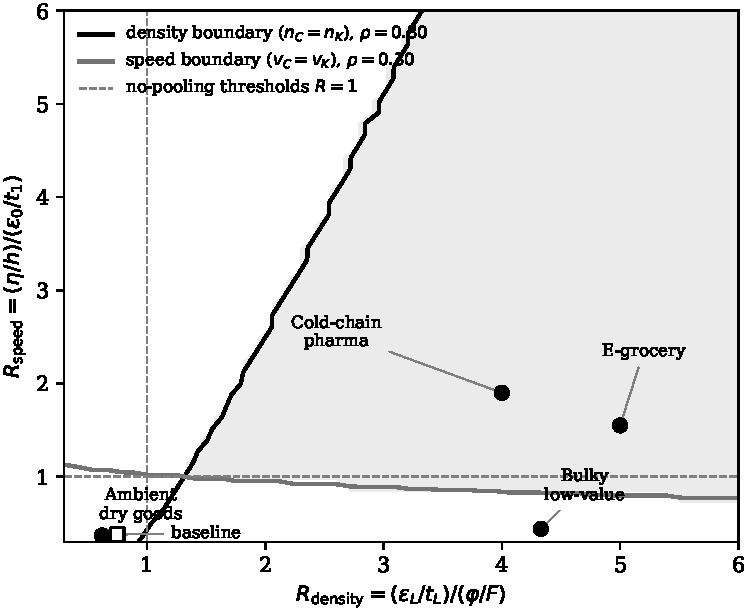
\includegraphics[width=0.70\linewidth]{fig_regimes.pdf}
\caption{Computed regime boundaries in the plane of the two carbon-intensity-per-dollar ratios. Solid curves
are the speed boundary ($v_C=v_K$) and the density boundary ($n_C=n_K$) at $\rho=0.30$; dashed lines are the
no-pooling thresholds $R_{\mathrm{speed}}=1$ and $R_{\mathrm{density}}=1$. The pooling-adjusted density
boundary tilts further right as $R_{\mathrm{speed}}$ rises, lying to the right of $R_{\mathrm{density}}=1$
where $\eta/h>\varphi/F$ and near or left of it otherwise, tracing the mediant of \eqref{eq:densthreshpool}. The shaded region is the faster-and-more-dispersed regime;
points locate the four archetypes of Table~\ref{tab:archcalib} and the baseline.}
\label{fig:regimes}
\end{figure}

\subsection{Constructing the product archetypes}

The four archetypes are guided by external benchmarks. Their two diagnostic ratios are
carbon intensities per dollar, whose components are measurable, and Table~\ref{tab:calibemp} maps published
emission factors and costs into those ratios. The emission factors are well established (national inventories
and standard conversion-factor sets) and the cost figures order-of-magnitude (industry benchmarks), so the
benchmarks set the \emph{relative} magnitudes of the ratios across archetypes rather than estimate parameters.

\begin{table}[t]
\centering\small
\setlength{\tabcolsep}{4pt}
\caption{From published benchmarks to the model's diagnostic ratios. Emission factors are from national
inventories and conversion-factor sets (high confidence); costs are industry benchmarks
(order-of-magnitude). The final column lists the archetypes each anchor informs.}
\label{tab:calibemp}
\begin{tabular}{@{}>{\raggedright\arraybackslash}p{0.21\linewidth}
                   >{\raggedright\arraybackslash}p{0.27\linewidth}
                   >{\raggedright\arraybackslash}p{0.30\linewidth}
                   >{\raggedright\arraybackslash}p{0.14\linewidth}@{}}
\toprule
Empirical anchor & Observed pattern & Model implication & Archetypes \\
\midrule
Warehouse energy, cold vs.\ ambient \citep{energystar2024medians, epa2025egrid}
 & refrigerated $\approx 3.7\times$ ambient carbon ($\approx 8.6$ vs.\ $2.3$ kg CO$_2$e/ft$^2$/yr)
 & raises holding carbon $\eta$, so larger $\eta/h$ (favors faster replenishment)
 & cold-chain, e-grocery \\
\addlinespace
Last-mile van vs.\ HGV \citep{defra2024ghg, defra2024methodology, glec2022framework}
 & van $\approx 0.62$ kg CO$_2$e/t-km, $\approx 6$--$8\times$ HGV, $37$--$41\%$ fill
 & raises last-mile $\varepsilon_L$, so larger $\varepsilon_L/t_L$ (favors dispersion)
 & e-grocery, pharma, bulky \\
\addlinespace
Bulky, ambient, low-value \citep{usgs2025stone}
 & crushed stone $\approx \$17.5$/tonne; minimal, inexpensive storage
 & low storage carbon keeps $\eta/h$ low; dispersion is driven by high $\varepsilon_L/t_L$, not $\eta/h$
 & bulky low-value \\
\addlinespace
High value density \citep{faf2023framework}
 & pharma $\approx \$49{,}000$/tonne
 & large $h$ damps $\eta/h$; pharma's high $\eta/h$ relies on cold-chain/compliance energy dominating $h$
 & cold-chain pharma \\
\addlinespace
Line-haul mode factors \citep{defra2025ghg}
 & ocean $0.016 <$ rail $0.028 <$ road $0.10$--$0.21$ kg CO$_2$e/t-km
 & orders inbound carbon against speed; $\varepsilon_0/t_1$ not identified
 & inbound (all) \\
\bottomrule
\end{tabular}
\end{table}

The two strongest anchors (Table~\ref{tab:calibemp}) are the refrigerated-warehouse energy premium, which
places cold-chain and e-grocery in the high-$\eta/h$ band, and the low-fill diesel last mile, which raises
$\varepsilon_L/t_L$ and underlies the load-factor result reported below. Value density enters through the holding cost, since the capital cost of inventory is
part of $h$: a higher-value product carries a larger $h$ and, at equal carbon, a smaller $\eta/h$. Cold-chain
pharma is therefore the one archetype whose holding placement is assumption-dependent: its high value density
enlarges $h$, so its high $\eta/h$ relies on the cold-chain energy and compliance component (refrigeration,
ultra-low-temperature, continuous monitoring) dominating the capital-cost denominator.

Using these anchors, we choose the normalized carbon-intensity ratios in Table~\ref{tab:archcalib}, which span
the four theoretical regimes; these values are regime-representative calibrations consistent with the relative
magnitudes above.

\begin{table}[t]
\centering\small
\caption{Carbon-intensity-per-dollar ratios for the four archetypes --- representative calibrations for the
four regimes --- and the diagnostics $R_{\mathrm{speed}}=(\eta/h)/(\varepsilon_0/t_1)$ and
$R_{\mathrm{density}}=(\varepsilon_L/t_L)/(\varphi/F)$ they imply.}
\label{tab:archcalib}
\begin{tabular}{@{}lcccccc@{}}
\toprule
Archetype & $\eta/h$ & $\varepsilon_0/t_1$ & $\varepsilon_L/t_L$ & $\varphi/F$
 & $R_{\mathrm{speed}}$ & $R_{\mathrm{density}}$\\
\midrule
Ambient dry goods    & $0.30$ & $0.80$ & $0.25$ & $0.40$ & $0.375$ & $0.625$\\
Cold-chain pharma    & $0.95$ & $0.50$ & $1.40$ & $0.35$ & $1.90$ & $4.00$\\
Bulky low-value      & $0.20$ & $0.45$ & $1.30$ & $0.30$ & $0.44$ & $4.33$\\
E-grocery perishable & $0.85$ & $0.55$ & $1.50$ & $0.30$ & $1.55$ & $5.00$\\
\bottomrule
\end{tabular}
\end{table}

\subsection{Product archetypes}

Table~\ref{tab:archetypes} reports the carbon-minimizing configuration for the four archetypes constructed
above. Because they share the cost rates, all four have the same cost-minimizing configuration ($n^*=7.8$,
$v^*=1.03$) and differ only in the direction and magnitude by which the carbon-minimizing configuration
departs from it. Slowing and consolidating is carbon-minimizing for the ambient dry-goods archetype; the
cold-chain and e-grocery archetypes call for faster and more dispersed networks; and the bulky, low-value
archetype, with inexpensive storage but a carbon-intensive last mile, disperses while slowing. Available
abatement ranges from about $6\%$ to $17\%$ of total carbon across the four; reaching $80\%$ of that abatement
costs between $0.5\%$ and $2.2\%$, while reaching the carbon minimum costs between $1.5\%$ and $7.8\%$, the
larger premiums attaching to the products that disperse most. All four archetypes have interior density optima
($J_n(1)<0<J_n(N)$), so none is a corner solution.

\begin{table}[t]
\centering\small
\setlength{\tabcolsep}{4.5pt}
\caption{Carbon-minimizing outcomes for the four archetypes calibrated in Table~\ref{tab:archcalib}: the
direction relative to the cost optimum, the largest attainable carbon reduction (``Max.\ reduction''), and the cost
premium to reach $80\%$ of that reduction and to reach the carbon minimum.}
\label{tab:archetypes}
\begin{tabular}{@{}llccc@{}}
\toprule
Archetype & Carbon-min direction & Max.\ reduction & Cost @ $80\%$ & Cost @ min\\
\midrule
Ambient dry goods    & slower, consolidate & $6.1\%$  & $+0.5\%$ & $+1.5\%$\\
Cold-chain pharma    & faster, disperse    & $7.7\%$  & $+1.1\%$ & $+3.8\%$\\
Bulky low-value      & slower, disperse    & $17.4\%$ & $+2.2\%$ & $+7.8\%$\\
E-grocery perishable & faster, disperse    & $9.6\%$  & $+1.4\%$ & $+4.8\%$\\
\bottomrule
\end{tabular}
\end{table}

\subsection{Value of joint redesign}

The two levers are complements (Proposition~\ref{prop:complement}); in this illustration, adjusting them together reaches
abatement levels and target costs that neither single-lever adjustment reaches. Table~\ref{tab:joint} reports this for a product in
the faster-and-more-dispersed regime (e-grocery perishables, $R_{\mathrm{speed}}=1.55$,
$R_{\mathrm{density}}=5.0$). Holding the network fixed and varying only speed lowers carbon by at most
$0.5\%$; holding speed fixed and varying only density reaches $8.4\%$; adjusting both reaches $9.6\%$. We
report two targets: a \emph{moderate} target of $7.6\%$, set at $90\%$ of the best single lever's attainable
abatement (here density, $0.90\times8.4\%$), and a \emph{deep} target of $9.1\%$, set at $95\%$ of the joint
attainable abatement ($0.95\times9.6\%$). The moderate target is infeasible on the speed lever alone and costs
$1.8\%$ on the density lever alone, but only $1.3\%$ when both are adjusted; the deep target lies beyond either
single lever and is met only by adjusting both. Faster replenishment lowers the inventory penalty of
dispersing, so the joint redesign extends the reach of each lever.

\begin{table}[t]
\centering\small
\caption{Value of adjusting both levers, for the e-grocery archetype. ``Max.\ reduction'' is the largest carbon
reduction the policy attains; the last two columns give the cost increase to meet a moderate and a deep
carbon target.}
\label{tab:joint}
\begin{tabular}{@{}lccc@{}}
\toprule
Policy & Max carbon cut & Cost at $7.6\%$ target & Cost at $9.1\%$ target\\
\midrule
Speed only ($n$ fixed)   & $0.5\%$ & infeasible & infeasible\\
Density only ($v$ fixed) & $8.4\%$ & $+1.8\%$   & infeasible\\
Joint $(n,v)$            & $9.6\%$ & $+1.3\%$   & $+2.8\%$\\
\bottomrule
\end{tabular}
\end{table}

\subsection{Carbon-price path}

Figure~\ref{fig:frontier} traces the cost--carbon frontier as the carbon price $\tau$ rises from zero, for
the baseline product. The configuration shifts from the cost-minimizing point to the carbon-minimizing one,
with both levers moving inward together --- the network consolidates from $7.8$ to $6.6$ DCs and the speed
falls from $1.03$ to $0.69$ --- and most of the movement occurs at low prices, the frontier flattening as
the configuration approaches the carbon-minimizing one.

\begin{figure}[t]
\centering
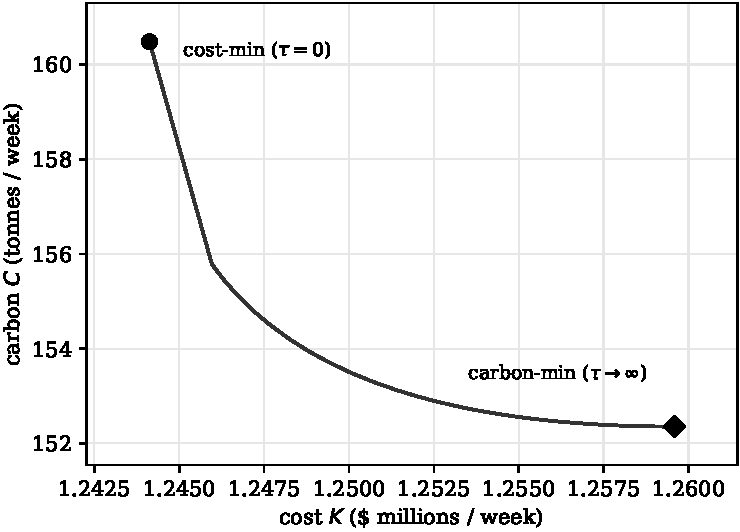
\includegraphics[width=0.64\linewidth]{fig_frontier.pdf}
\caption{Cost--carbon frontier for the baseline product, tracing the cost--carbon Pareto frontier as the
carbon price $\tau$ increases from $0$ to $\infty$. The endpoints
are the cost-minimizing ($\tau=0$) and carbon-minimizing ($\tau\to\infty$) configurations.}
\label{fig:frontier}
\end{figure}

\subsection{Chance-constrained carbon caps}

Moving from an expected carbon cap to a cap on \emph{realized} carbon held with high confidence is not merely
a tightening of the same constraint; by Proposition~\ref{prop:chance} it scales the transport component by
$m=1+z_{\beta_c}\,\mathrm{CV}_Q$ and so reweights transport emissions relative to inventory and facilities,
changing the relative attractiveness of speed and density. We trace this for the baseline product. With
$N=40$, $\mu=20{,}000$, $\sigma=8{,}000$ (CV $0.40$), and $\rho=0.30$, the aggregate throughput coefficient
of variation is
\[
  \mathrm{CV}_Q=\frac{\sigma}{\mu}\sqrt{\frac{1+(N-1)\rho}{N}}\approx 0.225,
\]
so the transport scalar is $m\approx 1.29$, $1.37$, and $1.52$ at the $90\%$, $95\%$, and $99\%$ confidence
levels ($z_{\beta_c}\approx 1.28,\,1.64,\,2.33$), against $m=1$ for the expected cap.

Table~\ref{tab:chance} reports the carbon-minimizing design under the scaled carbon function at each
confidence level, with $\varepsilon_0$ and $\varepsilon_L$ replaced by $m\varepsilon_0$ and $m\varepsilon_L$.
Two effects appear, consistent with Corollary~\ref{cor:chance}. On speed, the effective inbound ratio
$m\varepsilon_0/t_1$ rises from $0.80$ to $1.22$, moving further above the holding ratio $\eta/h=0.30$, so the
carbon-minimizing speed falls at every confidence level, from $0.69$ to $0.59$. On density, the effective
last-mile ratio $m\varepsilon_L/t_L$ rises from $0.30$ to $0.46$, raising the risk-weighted last-mile term
against the pooling-adjusted facility threshold of Proposition~\ref{prop:density}. That proposition compares
density best responses at a \emph{fixed} speed; the table instead reports the \emph{joint} carbon-minimizing
density $n_C$ against the joint cost-minimizing density $n_K$, in which the speed also adjusts. On that joint
basis the network shifts from more consolidated than the cost optimum (at the expected and $90\%$ caps) to
more dispersed (at the $95\%$ and $99\%$ caps), so the crossing of $n_K$ occurs between the $90\%$ and $95\%$
levels. For this product a high-confidence carbon cap therefore calls for a chain that is slower and
progressively less consolidated, and beyond a threshold confidence more dispersed than the cost optimum --- a
change in direction produced by the accounting rule alone, with the physical parameters held fixed.
Figure~\ref{fig:chance} traces the two designs across confidence levels.

\begin{table}[t]
\centering\small
\setlength{\tabcolsep}{4.5pt}
\caption{Effect of chance-constrained carbon accounting on the carbon-minimizing design (baseline product;
cost optimum $n_K=7.8$, $v_K=1.03$; reference thresholds $\eta/h=0.30$ and the no-pooling facility ratio
$\varphi/F=0.40$, against which the pooling-adjusted density threshold at the cost optimum is $\approx0.37$). ``Speed'' and
``Network'' give the direction relative to the cost optimum. Higher confidence scales the transport component by
$m$, lowering the carbon-minimizing speed and, beyond the $90\%$ level, dispersing the network.}
\label{tab:chance}
\begin{tabular}{@{}lcccccccc@{}}
\toprule
Cap / conf. & $m$ & $m\varepsilon_0/t_1$ & $m\varepsilon_L/t_L$ & $v_C$ & $n_C$ & Speed & Network & Cost prem.\\
\midrule
Expected ($m{=}1$) & $1.00$ & $0.80$ & $0.30$ & $0.69$ & $6.6$ & slower & consolidate & $+1.2\%$\\
$90\%$             & $1.29$ & $1.03$ & $0.39$ & $0.63$ & $7.7$ & slower & consolidate & $+1.7\%$\\
$95\%$             & $1.37$ & $1.10$ & $0.41$ & $0.62$ & $8.0$ & slower & disperse    & $+1.9\%$\\
$99\%$             & $1.52$ & $1.22$ & $0.46$ & $0.59$ & $8.6$ & slower & disperse    & $+2.2\%$\\
\bottomrule
\end{tabular}
\end{table}

\begin{figure}[t]
\centering
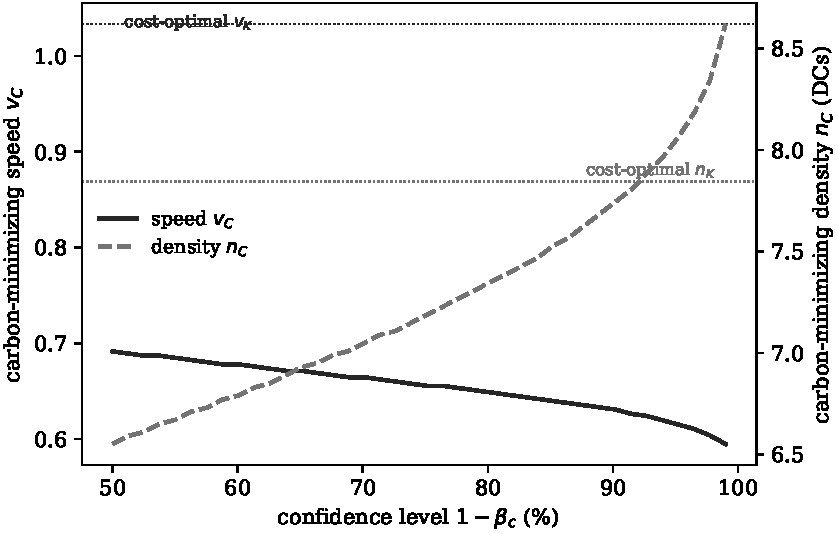
\includegraphics[width=0.64\linewidth]{fig_chance.pdf}
\caption{Carbon-minimizing speed $v_C$ (left axis, solid) and density $n_C$ (right axis, dashed) under
increasingly stringent confidence levels for the baseline product. Dotted lines mark the cost-optimal speed
$v_K$ and density $n_K$; the carbon-minimizing speed stays below $v_K$ throughout, while the carbon-minimizing
density rises through $n_K$ between the $90\%$ and $95\%$ confidence levels.}
\label{fig:chance}
\end{figure}

\noindent A high-confidence carbon cap changes the design calculation by placing a risk margin on transport
emissions: it makes faster replenishment less attractive, because inbound transport emissions receive a
higher effective weight, and it makes dispersion more attractive, because last-mile emissions receive a
higher effective weight. Two comparisons must be kept apart here. At a \emph{fixed} speed,
by Proposition~\ref{prop:density} the density best response exceeds the cost optimum once the risk-scaled
last-mile ratio $m\,\varepsilon_L/t_L$ clears the pooling-adjusted threshold ($\approx0.37$ at the cost
optimum, below the no-pooling divider $\varphi/F=0.40$); by that fixed-speed test dispersion would already set
in at the $90\%$ cap, where $m\,\varepsilon_L/t_L=0.39$. The table and Figure~\ref{fig:chance}, however,
report the \emph{joint} carbon-minimizing density $n_C$ against the joint cost optimum $n_K$, and the risk
margin also lowers the speed; by complementarity (Proposition~\ref{prop:complement}) a slower chain calls for
fewer warehouses, which partly offsets the dispersion. The net effect is that the joint $n_C$ rises through
$n_K$ only between the $90\%$ and $95\%$ levels --- later than the fixed-speed crossing. The fixed-speed
threshold and the joint crossing are thus distinct and should not be equated. Demand uncertainty enters the
carbon design through two channels: safety stock on the inventory side and a throughput-risk margin on the
transport side.

\paragraph{Sensitivity to demand variability.} The transport scalar $m=1+z_{\beta_c}\,\mathrm{CV}_Q$ rises with
the demand coefficient of variation, since $\mathrm{CV}_Q=(\sigma/\mu)\sqrt{[1+(N-1)\rho]/N}$ is increasing in
$\sigma/\mu$. Table~\ref{tab:chancecv} repeats the $95\%$ cap at three demand CVs. A more variable demand
raises $m$ --- from $1.19$ at $\mathrm{CV}=0.20$ to $1.56$ at $\mathrm{CV}=0.60$ --- and so deepens the
transport reweighting and the reduction in carbon-minimizing speed. The carbon-minimizing density at the
$95\%$ cap is roughly flat near eight DCs, while the cost optimum consolidates as variability grows (more
safety stock raises the value of pooling), so relative to the cost optimum the high-confidence network is
more consolidated at low CV and more dispersed at high CV.

\begin{table}[t]
\centering\small
\caption{Chance-constrained cap at $95\%$ confidence across demand variability. Higher demand CV raises the
throughput-risk scalar $m$; the network direction is stated relative to the (CV-dependent) cost optimum.}
\label{tab:chancecv}
\begin{tabular}{@{}cccccc@{}}
\toprule
Demand CV & $\mathrm{CV}_Q$ & cost opt.\ $(n_K,v_K)$ & $m$ at $95\%$ & carbon-min $(n_C,v_C)$ & Network vs.\ cost\\
\midrule
$0.20$ & $0.113$ & $(8.7,\,0.79)$ & $1.19$ & $(8.0,\,0.50)$ & consolidate\\
$0.40$ & $0.225$ & $(7.8,\,1.03)$ & $1.37$ & $(8.0,\,0.62)$ & disperse\\
$0.60$ & $0.338$ & $(7.2,\,1.21)$ & $1.56$ & $(8.1,\,0.69)$ & disperse\\
\bottomrule
\end{tabular}
\end{table}

\paragraph{Monte Carlo check.} Because the chance constraint has a deterministic equivalent, no
simulation is needed to solve it; a Monte Carlo check nonetheless confirms that the normal approximation
delivers the intended coverage. Fixing the design at the cost optimum and setting the cap at the normal
deterministic equivalent for each confidence level, we draw $5\times10^5$ realizations of aggregate throughput
and record the empirical frequency with which realized carbon exceeds the cap (Table~\ref{tab:mc}). Under
normally distributed throughput the empirical violation rate matches the nominal $\beta_c$ to within sampling
error, confirming the algebra of Proposition~\ref{prop:chance}. Under right-skewed (gamma) throughput of equal
mean and variance the violation rate exceeds the nominal level, and the gap widens at higher confidence and
higher CV --- the $99\%$ cap admits a $1.9\%$ violation at $\mathrm{CV}=0.40$ and $2.6\%$ at
$\mathrm{CV}=0.80$ --- so a firm facing strongly skewed demand should set $z_{\beta_c}$ from the empirical
throughput quantile rather than the normal one, as the distribution-free form of Proposition~\ref{prop:chance}
permits.

\begin{table}[t]
\centering\small
\caption{Monte Carlo check of the chance constraint ($5\times10^5$ draws; design fixed at the cost
optimum, cap at the normal deterministic equivalent). Empirical violation frequency $\Pr\{\tilde C>B\}$ under
normal and right-skewed (gamma) throughput of equal mean and variance.}
\label{tab:mc}
\begin{tabular}{@{}lccc@{}}
\toprule
 & Nominal $\beta_c$ & Normal demand & Gamma demand\\
\midrule
\multicolumn{4}{@{}l}{\emph{Demand CV $=0.40$ ($\mathrm{CV}_Q=0.225$)}}\\
\quad $90\%$ cap & $0.100$ & $0.100$ & $0.105$\\
\quad $95\%$ cap & $0.050$ & $0.050$ & $0.061$\\
\quad $99\%$ cap & $0.010$ & $0.010$ & $0.019$\\
\addlinespace
\multicolumn{4}{@{}l}{\emph{Demand CV $=0.80$ ($\mathrm{CV}_Q=0.451$)}}\\
\quad $90\%$ cap & $0.100$ & $0.100$ & $0.108$\\
\quad $95\%$ cap & $0.050$ & $0.050$ & $0.068$\\
\quad $99\%$ cap & $0.010$ & $0.010$ & $0.026$\\
\bottomrule
\end{tabular}
\end{table}

\subsection{Robustness}

The robustness analysis comprises four checks. Table~\ref{tab:robust} reports the first three. Restricting the
network to an integer number of DCs returns the continuous result rounded (cost eight, carbon seven).
Restricting replenishment to three discrete modes ($v\in\{0.5,1.0,2.0\}$) leaves the cost optimum at the
standard mode and shifts the carbon optimum to the slow mode, the discrete counterpart of the continuous speed
reduction. Varying the demand correlation $\rho$ shifts both optima toward more facilities as pooling weakens,
with the carbon optimum consolidated relative to the cost optimum throughout. The fourth check, reported
separately in Table~\ref{tab:loadfactor}, applies a reduced-form last-mile carbon rate that falls with vehicle
fill, $\varepsilon_L\,[\,0.5+0.5\,(n/n_{\mathrm{ref}})\,]$ with $n_{\mathrm{ref}}=8$ (half load-sensitive at the
reference density), adding a transport benefit of consolidation: it lowers the carbon-minimizing density
sharply, from $6.6$ to $3.0$ DCs for the baseline and from $22.8$ to $5.8$ for the bulky archetype. The dispersion conclusions are
therefore conditional on shipment-size-independent transport rates; load-sensitive rates shift the boundary
toward consolidation.

\begin{table}[t]
\centering\small
\caption{Robustness of the baseline cost- and carbon-minimizing designs to integer density, discrete speed
modes, and demand correlation. Entries are $(n,v)$ except the correlation rows, which report density $n$.}
\label{tab:robust}
\begin{tabular}{@{}lcc@{}}
\toprule
Variation & Cost-min & Carbon-min\\
\midrule
Continuous baseline               & $(7.8,\,1.03)$ & $(6.6,\,0.69)$\\
Integer $n$                       & $(8,\,1.04)$   & $(7,\,0.69)$\\
Discrete modes $v\in\{0.5,1,2\}$  & $(7.8,\,1.0)$  & $(6.3,\,0.5)$\\
\addlinespace
Correlation $\rho=0.0$            & $n=5.9$ & $n=4.8$\\
Correlation $\rho=0.3$            & $n=7.8$ & $n=6.6$\\
Correlation $\rho=0.6$            & $n=8.9$ & $n=7.4$\\
Correlation $\rho=0.9$            & $n=9.8$ & $n=8.1$\\
\bottomrule
\end{tabular}
\end{table}

\begin{table}[t]
\centering\small
\caption{Load-factor sensitivity. Under a reduced-form last-mile carbon rate that falls with vehicle fill,
$\varepsilon_L\,[\,0.5+0.5\,(n/n_{\mathrm{ref}})\,]$ with $n_{\mathrm{ref}}=8$, fuller vehicles under
consolidation lower the carbon-minimizing density; for the bulky archetype this reverses the dispersion of
Table~\ref{tab:archetypes}.}
\label{tab:loadfactor}
\begin{tabular}{@{}lcc@{}}
\toprule
 & Carbon-min $n$, constant rate & Carbon-min $n$, load-sensitive\\
\midrule
Baseline product           & $6.6$  & $3.0$\\
Bulky low-value archetype  & $22.8$ & $5.8$\\
\bottomrule
\end{tabular}
\end{table}

% =====================================================================
\section{Managerial Implications}\label{sec:managerial}

The carbon-minimizing configuration of speed and density depends on the two carbon-intensity-per-dollar
comparisons established in Section~\ref{sec:analysis}: holding against inbound transport, which governs speed,
and last-mile delivery against facilities, which governs density. Table~\ref{tab:regimes} arranges the four
combinations; slowing and consolidating --- the common transport levers --- correspond to the lower-left cell,
and the carbon-minimizing direction differs in the other three. The split on density uses the facility
comparison; under pooling the dividing line shifts toward the holding comparison
(Proposition~\ref{prop:density}), so, when holding is more carbon-intensive per dollar than facilities ($\eta/h>\varphi/F$), a strongly pooled network needs a more carbon-intensive last mile to justify dispersing.

\begin{table}[t]
\centering\small
\caption{Direction the carbon-minimizing configuration shifts relative to the cost optimum, by the two
carbon-intensity-per-dollar comparisons. The density columns split at the facility comparison; under risk
pooling the dividing line is the pooling-adjusted threshold of Proposition~\ref{prop:density}, which lies
between the facility and holding comparisons, so the facility comparison is a reference, not the exact
boundary.}
\label{tab:regimes}
\renewcommand{\arraystretch}{1.25}
\begin{tabular}{@{}>{\raggedright\arraybackslash}p{0.18\linewidth}
                   >{\raggedright\arraybackslash}p{0.36\linewidth}
                   >{\raggedright\arraybackslash}p{0.36\linewidth}@{}}
\toprule
 & \textbf{Lower network density}\newline {\small\itshape last mile less carbon-intensive per dollar than facilities} & \textbf{Higher network density}\newline {\small\itshape last mile more carbon-intensive per dollar than facilities} \\
\midrule
\textbf{Higher replenishment speed}\newline {\small\itshape holding more carbon-intensive per dollar than inbound transport}
  & faster and more consolidated, pooling inventory upstream --- carbon-intensive inventory with a lower-emission or short last mile
  & \emph{faster and more dispersed} --- cold-chain, volatile, high-service goods on a diesel last mile \\
\textbf{Lower replenishment speed}\newline {\small\itshape holding less carbon-intensive per dollar than inbound transport}
  & slower and more consolidated --- the transport-lever case; ambient, stable, low-service dry goods
  & slower long haul, denser network --- lower-emission, low-cost storage with carbon-intensive inbound and last mile \\
\bottomrule
\end{tabular}
\end{table}

\paragraph{Diagnosis.} The two ratios, computed for a given product, locate it in one cell of
Table~\ref{tab:regimes}, which indicates the carbon-minimizing direction of speed and density. A uniform
policy of slowing replenishment and consolidating the network coincides with the carbon-minimizing
configuration only for products in the lower-left cell.

\paragraph{A decision procedure.} The diagnosis suggests a concrete sequence for a firm holding a carbon target.
\emph{(i)} From its own rate data, estimate each activity's carbon intensity per dollar --- for holding,
inbound transport, last-mile delivery, and facilities. \emph{(ii)} For speed, compare holding with inbound
transport: if holding is the more carbon-intensive per dollar, the carbon-minimizing direction is faster
replenishment, and otherwise slower (Proposition~\ref{prop:speed}). \emph{(iii)} For density, compare
last-mile delivery with the pooling-adjusted facility threshold of Proposition~\ref{prop:density} rather than
with facilities alone --- pooling shifts the threshold from $\varphi/F$ toward the holding ratio $\eta/h$, so
stronger pooling raises the bar for dispersing when $\eta/h>\varphi/F$. \emph{(iv)} These comparisons give the carbon-minimizing \emph{direction} on each axis,
not a single-lever implementation rule: because the levers are complements, set the two together rather than
in sequence, since the chosen speed raises or lowers the value of dispersing, and conversely. \emph{(v)} If the
cap is on realized rather than expected carbon, inflate the transport intensities by the throughput risk
margin (Proposition~\ref{prop:chance}) before applying steps (ii)--(iii).

\paragraph{Replenishment speed.} For refrigerated, volatile, or high-service products --- those for which
inventory is the emissions-intensive component --- a tighter carbon target is met by shipping \emph{faster},
because the safety stock that a slower mode would require carries more carbon than the faster transport adds.
This case corresponds to the top row of Table~\ref{tab:regimes}.

\paragraph{Consolidation and the last mile.} Consolidation lowers carbon here
through inventory pooling and reduced facility energy while lengthening the last mile. A firm whose last
mile is carbon-intensive --- diesel vans, long rural routes --- can lower total carbon by holding more stock
nearer to demand, even though that raises total inventory; the transport channel of consolidation works
against it. This last channel is strong when vehicle fill improves with consolidation: under a load-sensitive
last mile the carbon-minimizing network can swing sharply back toward consolidation --- for the bulky
archetype, from $22.8$ to $5.8$ DCs (Section~\ref{sec:numerical}) --- so a firm should weigh its last mile's
load sensitivity before dispersing.

\paragraph{Joint adjustment of the two levers.} Because the levers are complements, a program that adjusts
only one --- a slow-steaming mandate or a network-consolidation initiative --- attains part of the available
abatement, and for some products shifts a lever away from its carbon-minimizing direction. The cost of working
one lever at a time is quantifiable: for the e-grocery archetype (Section~\ref{sec:numerical},
Table~\ref{tab:joint}), adjusting speed alone abates at most $0.5\%$ and density alone $8.4\%$, while adjusting
both reaches $9.6\%$, and a target of $7.6\%$ that costs $1.8\%$ on the density lever alone costs only $1.3\%$
when both are adjusted. Joint redesign can thus expand the abatement reach and, in this illustration, it lowers the cost
of meeting the target relative to single-lever adjustment, which supports evaluating the two levers together.

\paragraph{Product segmentation, service, and volatility.} Because the carbon-minimizing configuration
depends on the product, a single chain-wide policy serves a heterogeneous portfolio imperfectly. The
service-level target and demand variability also bear on carbon: a higher service-level target and a more
volatile demand both enlarge safety stock and so, by Proposition~\ref{prop:service}, raise the
carbon-minimizing speed and strengthen the pull toward consolidation through the value of pooling, unless the
last-mile comparison dominates the density decision. A $99\%$ cycle-service target is thus a carbon-design
parameter, not only an inventory-cost one. Higher demand correlation across markets weakens the pooling
benefit that favors consolidation and can make dispersion more attractive, so forecasting and
demand-smoothing are carbon levers in their own right.

\paragraph{Carbon accounting and confidence.} Whether the cap is placed on expected or on realized carbon is
itself a design parameter. A cap on realized carbon held with high confidence places a risk margin on
transport emissions (Proposition~\ref{prop:chance}); by Corollary~\ref{cor:chance} this tightens the speed
threshold --- making faster replenishment harder to justify on carbon grounds --- and relaxes the dispersion
threshold, so a firm facing a high-confidence cap should reassess its configuration against the adjusted
thresholds. For the baseline product, raising the confidence level lowers the
carbon-minimizing speed at every level and, beyond a threshold confidence, shifts the network from
consolidation to dispersion relative to the cost optimum (Section~\ref{sec:numerical},
Table~\ref{tab:chance}); whether that shift occurs depends on whether the risk-weighted last-mile term
overcomes the facility and pooling forces.

\paragraph{Implication for policy.} The two-component structure carries a caution for regulation. A rule that
prices or caps only transport leaves the holding component untouched and can induce substitution into inventory
and facilities to comply, raising emissions the rule does not measure. Instruments scoped to transport alone
--- a freight fuel levy, a mode-shift mandate, or a vehicle-emissions standard --- are exposed to this
leakage, whereas an instrument that prices a firm's total logistics carbon (for example, a scope-inclusive
carbon charge or a cap covering both warehousing and transport emissions) avoids it and lets the firm choose
the speed-and-density mix that minimizes carbon across transport and inventory together.

% =====================================================================
\section{Discussion and Conclusion}\label{sec:discussion}

A distribution network provides two services --- availability and proximity --- each of which can be supplied
through more than one operational substitute, and carbon-aware design turns on which substitute a carbon price
makes cheaper in emissions terms rather than on a single transport-centered response. The appropriate configuration
therefore depends on how a carbon price changes the relative cost of providing those two services. When inventory is the emissions-intensive
way to provide availability, carbon favors buying it with replenishment speed rather than with safety stock;
when the last mile is the emissions-intensive way to provide proximity, carbon favors buying it with
facilities rather than with distance. The contribution of the paper is to make these substitutions explicit
and to give the thresholds at which the carbon-minimizing substitute differs from the cost-minimizing one.

\paragraph{Theoretical contribution.} The model embeds an endogenous replenishment speed in a
location--inventory network. Speed sets the lead time, the lead time sets the safety stock, and the safety
stock carries carbon, so a faster network is more carbon-intensive in transport but less inventory-intensive. This
coupling produces the speed threshold $\eta/h>\varepsilon'(v_{\mathrm K})/t'(v_{\mathrm K})$
(Proposition~\ref{prop:speed}): when holding is more carbon-intensive per dollar than inbound transport at the
margin, the carbon-minimizing chain replenishes faster than the cost-minimizing one. The density decision adds
the proximity substitution, with a \emph{pooling-adjusted} threshold (Proposition~\ref{prop:density}) in which
last-mile intensity is compared not to the facility ratio $\varphi/F$ but to a weighted average of $\varphi/F$
and the holding ratio $\eta/h$, so risk pooling enters the boundary explicitly. The two levers are complements
(Proposition~\ref{prop:complement}): faster replenishment lowers the inventory penalty of dispersion, so the
optimal degree of centralization is itself contingent on speed. The chance-constrained extension
(Proposition~\ref{prop:chance}) preserves this structure: a cap on realized rather than expected carbon scales
the transport component by $m=q_{1-\beta_c}/(N\mu)$, leaving the four-component form and the comparative statics intact
while shifting both thresholds.

\paragraph{Managerial and policy implications.} For practice, the diagnostic is to measure carbon intensity
per dollar by activity and to locate each product in the resulting regime (Section~\ref{sec:managerial}).
Because the carbon-minimizing configuration depends on the product, a single chain-wide policy serves a
heterogeneous portfolio imperfectly, and service-level targets and demand volatility are carbon-design
parameters rather than inventory-cost parameters alone. In the e-grocery illustration, joint redesign expands
abatement reach and lowers the cost of the target relative to single-lever adjustment, and a high-confidence
carbon cap can alter the relative attractiveness of speed and dispersion. For policy, the two-component structure cautions that regulation aimed only at transport can
induce substitution into inventory and facility emissions that the rule does not measure; total logistics
carbon is the appropriate accounting boundary, and a chance-constrained or high-confidence target places
particular weight on the variability of transport throughput.

\paragraph{Limitations.} The model is deliberately parsimonious. Markets are symmetric and treated through a
continuous-approximation geometry; the setting is single-product; inbound distance is represented by a single
representative mean; our model carries no explicit vehicle load-factor decision; service is modeled
through a cycle service level rather than a fill rate; the expected-value cap is the baseline against which the
chance-constrained cap is compared; and the calibration is regime-representative rather than an empirical
estimation. Each abstraction trades realism for the closed-form structure that makes the substitutions
analytically tractable. Our model also abstracts from load-sensitive transport rates; the robustness checks show
that a load-sensitive last mile can attenuate or even reverse dispersion. The dispersion conclusions are thus
conditional on shipment-size-independent transport rates, and on the omission of inbound consolidation and
facility scale economies; each of these forces shifts the boundary toward consolidation.

\paragraph{Future research.} Several extensions follow naturally: multi-product portfolio design, in which a
shared network serves products with different carbon-intensity profiles; explicit load-factor and
shipment-consolidation emissions, which would add shipment size as a third lever; heterogeneous geography and
discrete facility locations in place of the continuous approximation; empirical calibration using firm-level
logistics-emissions data; endogenous service-level choice, which Proposition~\ref{prop:service} treats as a
fixed carbon parameter but which a fuller model would set jointly with speed and density, internalizing the
carbon cost of a service requirement; and multi-echelon safety-stock placement, which would couple the density and speed decisions
across more than one stocking tier.

Carbon-minimizing distribution design requires identifying the lower-emission
operational substitute for availability and for proximity. In some regimes that substitute is slower
replenishment and consolidation; in others it is faster replenishment, greater dispersion, or both. The model
provides a diagnostic structure --- two carbon-intensity-per-dollar comparisons, coupled through the
complementarity of speed and density --- for making that distinction.

\section*{Declaration of competing interest}
The author declares that he has no known competing financial interests or personal relationships that could
have appeared to influence the work reported in this paper.

\section*{Funding}
This research did not receive any specific grant from funding agencies in the public, commercial, or
not-for-profit sectors.

\section*{Data availability}
No data were used for the research described in the article. The code that generates all numerical
illustrations is available from the author on request.

\section*{CRediT authorship contribution statement}
\textbf{Ram Ganeshan:} Conceptualization, Methodology, Formal analysis, Software, Writing -- original draft,
Writing -- review \& editing.

\bibliographystyle{apalike}
\bibliography{references}

\end{document}
